% Options for packages loaded elsewhere
\PassOptionsToPackage{unicode}{hyperref}
\PassOptionsToPackage{hyphens}{url}
\PassOptionsToPackage{dvipsnames,svgnames,x11names}{xcolor}
\documentclass[
  10pt,
]{article}
\usepackage{xcolor}
\usepackage[a4paper,top=23mm,bottom=24mm,left=25mm,right=25mm]{geometry}
\usepackage{amsmath,amssymb}
\usepackage{graphicx}
\usepackage{tikz}
\usetikzlibrary{arrows.meta,positioning,calc}
\graphicspath{{docs/observatory/figures/}{figures/}}
\setcounter{secnumdepth}{5}
\usepackage{iftex}
\ifPDFTeX
  \usepackage[T1]{fontenc}
  \usepackage[utf8]{inputenc}
  \usepackage{textcomp} % provide euro and other symbols
\else % if luatex or xetex
  \usepackage{unicode-math} % this also loads fontspec
  \defaultfontfeatures{Scale=MatchLowercase}
  \defaultfontfeatures[\rmfamily]{Ligatures=TeX,Scale=1}
\fi
\usepackage{lmodern}
\ifPDFTeX\else
  % xetex/luatex font selection
\fi
% Use upquote if available, for straight quotes in verbatim environments
\IfFileExists{upquote.sty}{\usepackage{upquote}}{}
\IfFileExists{microtype.sty}{% use microtype if available
  \usepackage[]{microtype}
  \UseMicrotypeSet[protrusion]{basicmath} % disable protrusion for tt fonts
}{}
\makeatletter
\@ifundefined{KOMAClassName}{% if non-KOMA class
  \IfFileExists{parskip.sty}{%
    \usepackage{parskip}
  }{% else
    \setlength{\parindent}{0pt}
    \setlength{\parskip}{6pt plus 2pt minus 1pt}}
}{% if KOMA class
  \KOMAoptions{parskip=half}}
\makeatother
\usepackage{color}
\usepackage{fancyvrb}
\newcommand{\VerbBar}{|}
\newcommand{\VERB}{\Verb[commandchars=\\\{\}]}
\DefineVerbatimEnvironment{Highlighting}{Verbatim}{commandchars=\\\{\}}
% Add ',fontsize=\small' for more characters per line
\newenvironment{Shaded}{}{}
\newcommand{\AlertTok}[1]{\textcolor[rgb]{1.00,0.00,0.00}{\textbf{#1}}}
\newcommand{\AnnotationTok}[1]{\textcolor[rgb]{0.38,0.63,0.69}{\textbf{\textit{#1}}}}
\newcommand{\AttributeTok}[1]{\textcolor[rgb]{0.49,0.56,0.16}{#1}}
\newcommand{\BaseNTok}[1]{\textcolor[rgb]{0.25,0.63,0.44}{#1}}
\newcommand{\BuiltInTok}[1]{\textcolor[rgb]{0.00,0.50,0.00}{#1}}
\newcommand{\CharTok}[1]{\textcolor[rgb]{0.25,0.44,0.63}{#1}}
\newcommand{\CommentTok}[1]{\textcolor[rgb]{0.38,0.63,0.69}{\textit{#1}}}
\newcommand{\CommentVarTok}[1]{\textcolor[rgb]{0.38,0.63,0.69}{\textbf{\textit{#1}}}}
\newcommand{\ConstantTok}[1]{\textcolor[rgb]{0.53,0.00,0.00}{#1}}
\newcommand{\ControlFlowTok}[1]{\textcolor[rgb]{0.00,0.44,0.13}{\textbf{#1}}}
\newcommand{\DataTypeTok}[1]{\textcolor[rgb]{0.56,0.13,0.00}{#1}}
\newcommand{\DecValTok}[1]{\textcolor[rgb]{0.25,0.63,0.44}{#1}}
\newcommand{\DocumentationTok}[1]{\textcolor[rgb]{0.73,0.13,0.13}{\textit{#1}}}
\newcommand{\ErrorTok}[1]{\textcolor[rgb]{1.00,0.00,0.00}{\textbf{#1}}}
\newcommand{\ExtensionTok}[1]{#1}
\newcommand{\FloatTok}[1]{\textcolor[rgb]{0.25,0.63,0.44}{#1}}
\newcommand{\FunctionTok}[1]{\textcolor[rgb]{0.02,0.16,0.49}{#1}}
\newcommand{\ImportTok}[1]{\textcolor[rgb]{0.00,0.50,0.00}{\textbf{#1}}}
\newcommand{\InformationTok}[1]{\textcolor[rgb]{0.38,0.63,0.69}{\textbf{\textit{#1}}}}
\newcommand{\KeywordTok}[1]{\textcolor[rgb]{0.00,0.44,0.13}{\textbf{#1}}}
\newcommand{\NormalTok}[1]{#1}
\newcommand{\OperatorTok}[1]{\textcolor[rgb]{0.40,0.40,0.40}{#1}}
\newcommand{\OtherTok}[1]{\textcolor[rgb]{0.00,0.44,0.13}{#1}}
\newcommand{\PreprocessorTok}[1]{\textcolor[rgb]{0.74,0.48,0.00}{#1}}
\newcommand{\RegionMarkerTok}[1]{#1}
\newcommand{\SpecialCharTok}[1]{\textcolor[rgb]{0.25,0.44,0.63}{#1}}
\newcommand{\SpecialStringTok}[1]{\textcolor[rgb]{0.73,0.40,0.53}{#1}}
\newcommand{\StringTok}[1]{\textcolor[rgb]{0.25,0.44,0.63}{#1}}
\newcommand{\VariableTok}[1]{\textcolor[rgb]{0.10,0.09,0.49}{#1}}
\newcommand{\VerbatimStringTok}[1]{\textcolor[rgb]{0.25,0.44,0.63}{#1}}
\newcommand{\WarningTok}[1]{\textcolor[rgb]{0.38,0.63,0.69}{\textbf{\textit{#1}}}}
\usepackage{longtable,booktabs,array}
\newcolumntype{L}[1]{>{\raggedright\arraybackslash}p{#1}}
\usepackage{caption}
\usepackage{float}
\captionsetup{
  font=small,
  labelfont=bf,
  labelsep=period,
  justification=raggedright,
  singlelinecheck=false}
\captionsetup[table]{skip=7pt}
\newcounter{none} % for unnumbered tables
\usepackage{calc} % for calculating minipage widths
% Correct order of tables after \paragraph or \subparagraph
\usepackage{etoolbox}
\makeatletter
\patchcmd\longtable{\par}{\if@noskipsec\mbox{}\fi\par}{}{}
\makeatother
% Allow footnotes in longtable head/foot
\IfFileExists{footnotehyper.sty}{\usepackage{footnotehyper}}{\usepackage{footnote}}
\makesavenoteenv{longtable}
\setlength{\emergencystretch}{3em} % prevent overfull lines
\providecommand{\tightlist}{%
  \setlength{\itemsep}{0pt}\setlength{\parskip}{0pt}}
\usepackage{bookmark}
\usepackage{fancyhdr}
\IfFileExists{xurl.sty}{\usepackage{xurl}}{} % add URL line breaks if available
\urlstyle{same}
% fallback for those not using the hyperref driver hyperxmp:
\makeatletter
\@ifundefined{xmpquote}{\newcommand{\xmpquote}[1]{#1}}{}
\makeatother
\definecolor{OSGInk}{HTML}{17324D}
\definecolor{OSGRule}{HTML}{7F8C99}
\hypersetup{
  pdftitle={Open Selection Graph (OSG): a dataset for mapping observable populations and selection processes in science},
  pdfauthor={Anton Waagaard},
  colorlinks=true,
  linkcolor={OSGInk},
  filecolor={Maroon},
  citecolor={Blue},
  urlcolor={OSGInk},
  pdfcreator={Tectonic LaTeX}}

% Standalone Data Descriptor layout. Scientific Data requests a single
% self-contained TeX manuscript instead of an external journal class.
\setlength{\parindent}{0pt}
\setlength{\parskip}{0.58em plus 0.12em minus 0.08em}
\setlength{\columnsep}{7mm}
\renewcommand{\arraystretch}{1.12}
\pagestyle{fancy}
\fancyhf{}
\fancyhead[L]{\footnotesize\sffamily Open Selection Graph}
\fancyhead[R]{\footnotesize\sffamily Data Descriptor}
\fancyfoot[C]{\footnotesize\thepage}
\renewcommand{\headrulewidth}{0.35pt}
\renewcommand{\headrule}{\hbox to\headwidth{\color{OSGRule}\leaders\hrule height \headrulewidth\hfill}}
\setlength{\headheight}{19pt}

\makeatletter
\renewcommand\section{\@startsection{section}{1}{\z@}%
  {2.7ex \@plus 0.8ex \@minus 0.3ex}%
  {1.0ex \@plus 0.2ex}%
  {\normalfont\Large\sffamily\bfseries\color{OSGInk}}}
\renewcommand\subsection{\@startsection{subsection}{2}{\z@}%
  {2.2ex \@plus 0.6ex \@minus 0.2ex}%
  {0.8ex \@plus 0.2ex}%
  {\normalfont\large\sffamily\bfseries\color{OSGInk}}}
\renewcommand\subsubsection{\@startsection{subsubsection}{3}{\z@}%
  {1.8ex \@plus 0.5ex \@minus 0.2ex}%
  {0.6ex \@plus 0.1ex}%
  {\normalfont\normalsize\sffamily\bfseries\color{OSGInk}}}
\renewcommand{\maketitle}{%
  \thispagestyle{plain}%
  \begin{flushleft}%
    {\small\sffamily\bfseries\color{OSGInk} DATA DESCRIPTOR\par}%
    \vspace{0.55em}%
    {\color{OSGInk}\rule{\textwidth}{1.1pt}\par}%
    \vspace{1.0em}%
    {\fontsize{21}{25}\selectfont\sffamily\bfseries\color{OSGInk}\@title\par}%
    \vspace{1.15em}%
    {\large\sffamily\bfseries\@author\par}%
    \vspace{0.25em}%
    {\small\sffamily Dimensional Impact Lab\par}%
    {\small\sffamily\href{mailto:anton@dimpactlab.org}{anton@dimpactlab.org}\par}%
    \vspace{0.75em}%
    {\small\sffamily\color{OSGRule}\@date\par}%
    \vspace{0.75em}%
    {\color{OSGRule}\rule{\textwidth}{0.45pt}\par}%
  \end{flushleft}%
  \vspace{0.55em}%
}
\renewenvironment{abstract}{%
  \begin{minipage}{\textwidth}%
  {\sffamily\bfseries\color{OSGInk} Abstract\par}%
  \vspace{0.35em}\small
}{%
  \end{minipage}\par\vspace{0.7em}%
}
\makeatother

\IfFileExists{docs/observatory/generated/quantitative_claims.tex}
  {% Generated by observatory.r5; do not edit quantitative values by hand.
\providecommand{\OSGClaimAdmissibleRateCycles}{210}
\providecommand{\OSGClaimAfterlifeCandidates}{8,903}
\providecommand{\OSGClaimCandidateGateChains}{8,627}
\providecommand{\OSGClaimCommunityBenchmarkTasks}{6}
\providecommand{\OSGClaimConstructAtlasConstructs}{5}
\providecommand{\OSGClaimConstructAtlasRulers}{4}
\providecommand{\OSGClaimConstructAtlasSelectors}{9}
\providecommand{\OSGClaimConstructSpanAuditN}{314}
\providecommand{\OSGClaimConstructSpanPrecision}{1.0}
\providecommand{\OSGClaimConstructSpanPrecisionPercent}{100\%}
\providecommand{\OSGClaimConstructSpanPrecisionLower}{0.988}
\providecommand{\OSGClaimConstructSpanPrecisionLowerPercent}{98.79\%}
\providecommand{\OSGClaimEvaluationObjects}{40,483}
\providecommand{\OSGClaimExactEvaluationJoins}{40,102}
\providecommand{\OSGClaimFlowIdentityViolations}{12}
\providecommand{\OSGClaimFundingInstruments}{18}
\providecommand{\OSGClaimFundingPanelApplicationEvents}{21,883}
\providecommand{\OSGClaimFundingPanelChoiceSets}{1,521}
\providecommand{\OSGClaimFutureDatedExclusions}{450}
\providecommand{\OSGClaimHiddenScreenSensitivityRows}{34,104}
\providecommand{\OSGClaimHistoricalPolicyVersions}{4,531}
\providecommand{\OSGClaimHumanLineageConsensusPairs}{269}
\providecommand{\OSGClaimHumanLineageDecisivePairs}{284}
\providecommand{\OSGClaimHumanLineageKappa}{0.859}
\providecommand{\OSGClaimHumanLineageKappaPercent}{85.88\%}
\providecommand{\OSGClaimHumanLineageOofAuc}{0.971}
\providecommand{\OSGClaimHumanLineageOofAucPercent}{97.12\%}
\providecommand{\OSGClaimHumanReviewMaxAuc}{0.938}
\providecommand{\OSGClaimHumanReviewMaxAucPercent}{93.8\%}
\providecommand{\OSGClaimHumanReviewMinAuc}{0.72}
\providecommand{\OSGClaimHumanReviewMinAucPercent}{72\%}
\providecommand{\OSGClaimHumanReviewSpans}{13,724}
\providecommand{\OSGClaimHupdAcceptedApplications}{2,225,736}
\providecommand{\OSGClaimHupdPopulationCells}{578}
\providecommand{\OSGClaimHupdPublicApplications}{4,518,254}
\providecommand{\OSGClaimHupdRejectedApplications}{1,112,710}
\providecommand{\OSGClaimImmatureOutcomesExcluded}{113}
\providecommand{\OSGClaimInstitutionalGateCycles}{4,696}
\providecommand{\OSGClaimLineageAuditN}{711}
\providecommand{\OSGClaimLineagePrecision}{1.0}
\providecommand{\OSGClaimLineagePrecisionPercent}{100\%}
\providecommand{\OSGClaimLineagePrecisionLower}{0.995}
\providecommand{\OSGClaimLineagePrecisionLowerPercent}{99.46\%}
\providecommand{\OSGClaimLinkageCandidatePairs}{953}
\providecommand{\OSGClaimMatureObservationWindowRows}{32,510}
\providecommand{\OSGClaimModalCompletedReceipts}{12}
\providecommand{\OSGClaimModalSpendUsd}{26.782}
\providecommand{\OSGClaimModalSpendUsdPercent}{2678.18\%}
\providecommand{\OSGClaimObservabilityBoundCycles}{4,872}
\providecommand{\OSGClaimObservabilityCensusCycles}{4,872}
\providecommand{\OSGClaimObservabilityRecordedCountChanges}{9}
\providecommand{\OSGClaimObservabilityRecordedGradeChanges}{0}
\providecommand{\OSGClaimOpenreviewCurrentNotes}{679,898}
\providecommand{\OSGClaimOpenreviewForums}{44,330}
\providecommand{\OSGClaimOpenreviewPassingCycles}{176}
\providecommand{\OSGClaimOpenreviewRuleRecords}{4,525}
\providecommand{\OSGClaimPanoramaExactHupdMatches}{3,416}
\providecommand{\OSGClaimPanoramaHupdOverlapTwoZeroZeroFourTwoZeroOneSix}{0.915}
\providecommand{\OSGClaimPanoramaHupdOverlapTwoZeroZeroFourTwoZeroOneSixPercent}{91.49\%}
\providecommand{\OSGClaimPanoramaOutsideHupdYearBoundary}{3,532}
\providecommand{\OSGClaimPanoramaWithinHupdYearNonmatches}{1,195}
\providecommand{\OSGClaimPatentActionChains}{40,715}
\providecommand{\OSGClaimPatentCapacityCells}{3,391}
\providecommand{\OSGClaimPatentClaimAlignmentCoverage}{0.909}
\providecommand{\OSGClaimPatentClaimAlignmentCoveragePercent}{90.94\%}
\providecommand{\OSGClaimPatentClaimAlignmentRows}{174,120}
\providecommand{\OSGClaimPatentClaimAlignmentUnresolved}{15,777}
\providecommand{\OSGClaimPatentClaimStateAccountingCoverage}{1.0}
\providecommand{\OSGClaimPatentClaimStateAccountingCoveragePercent}{100\%}
\providecommand{\OSGClaimPatentFinalOnlyClaimStates}{15,548}
\providecommand{\OSGClaimPatentInitialOnlyClaimStates}{229}
\providecommand{\OSGClaimPatentPilotApplications}{8,143}
\providecommand{\OSGClaimPatentPriorArtLinks}{24,232}
\providecommand{\OSGClaimPointerRebuildArtifacts}{684}
\providecommand{\OSGClaimPolicySurfaceCycles}{4,522}
\providecommand{\OSGClaimPopulatedAdmissibleCycles}{200}
\providecommand{\OSGClaimProbabilisticBalancedPairs}{3,330}
\providecommand{\OSGClaimProbabilisticHighPrecisionPairs}{253}
\providecommand{\OSGClaimProbabilisticHighRecallPairs}{6,652}
\providecommand{\OSGClaimProbabilisticLinkageCandidates}{75,897}
\providecommand{\OSGClaimPublicObservabilitySnapshotRows}{410}
\providecommand{\OSGClaimPublicObservabilitySnapshots}{2}
\providecommand{\OSGClaimPublicationEventTimesUnidentified}{8,903}
\providecommand{\OSGClaimPublicationGateCycles}{350}
\providecommand{\OSGClaimPublicationLinkPrecision}{1.0}
\providecommand{\OSGClaimPublicationLinkPrecisionPercent}{100\%}
\providecommand{\OSGClaimPublicationLinkPrecisionLower}{0.989}
\providecommand{\OSGClaimPublicationLinkPrecisionLowerPercent}{98.94\%}
\providecommand{\OSGClaimPublicationLinkageBoundRows}{224}
\providecommand{\OSGClaimPublicationObservationWindowRows}{35,612}
\providecommand{\OSGClaimQwenThreeSemanticRows}{8,507}
\providecommand{\OSGClaimRecombinatorialVersions}{93}
\providecommand{\OSGClaimRecoverySourceCards}{53}
\providecommand{\OSGClaimRegisteredEstimands}{21}
\providecommand{\OSGClaimRegisteredReforms}{3}
\providecommand{\OSGClaimReleaseComponents}{6}
\providecommand{\OSGClaimReleaseParquetTables}{72}
\providecommand{\OSGClaimRepeatAwardeeLowerBounds}{1,555}
\providecommand{\OSGClaimReviewRateCycles}{197}
\providecommand{\OSGClaimRubricFields}{11,188}
\providecommand{\OSGClaimSchemaArtifacts}{26}
\providecommand{\OSGClaimSelectionRateCycles}{61}
\providecommand{\OSGClaimSemanticFeatureRows}{8,516}
\providecommand{\OSGClaimSemanticRulerCentroidSpearman}{0.554}
\providecommand{\OSGClaimSemanticRulerCentroidSpearmanPercent}{55.45\%}
\providecommand{\OSGClaimSemanticRulerMedianDisagreement}{0.167}
\providecommand{\OSGClaimSemanticRulerMedianDisagreementPercent}{16.7\%}
\providecommand{\OSGClaimSemanticRulerSharedRows}{8,501}
\providecommand{\OSGClaimSemanticVersions}{8,516}
\providecommand{\OSGClaimSnsfIndividualVoteCells}{4,811}
\providecommand{\OSGClaimSnsfOutcomeObservedProposals}{353}
\providecommand{\OSGClaimSnsfProposalPanelEvents}{432}
\providecommand{\OSGClaimSourceCards}{53}
\providecommand{\OSGClaimSourceDeclaredLineageEdges}{1,080}
\providecommand{\OSGClaimStageOutcomeAuditN}{7,255}
\providecommand{\OSGClaimStageOutcomePrecision}{1.0}
\providecommand{\OSGClaimStageOutcomePrecisionPercent}{100\%}
\providecommand{\OSGClaimTextualRecombinatorialCoverage}{0.927}
\providecommand{\OSGClaimTextualRecombinatorialCoveragePercent}{92.71\%}
\providecommand{\OSGClaimTextualRecombinatorialDocuments}{8,563}
\providecommand{\OSGClaimTextualRecombinatorialVersions}{7,939}
\providecommand{\OSGClaimTransportSourcePairs}{120}
\providecommand{\OSGClaimUkriOpportunities}{2,102}
\providecommand{\OSGClaimUkriPanelRounds}{1,449}
\providecommand{\OSGClaimUnmatchedAsNonpublication}{0}
\providecommand{\OSGClaimVerifiedOpenreviewCandidates}{55,369}
\providecommand{\OSGClaimVerifiedOpenreviewCycles}{176}
\providecommand{\OSGClaimVerifiedOpenreviewPopulatedCycles}{166}
\providecommand{\OSGClaimVerifiedOpenreviewReviews}{31,992}
\providecommand{\OSGClaimVersionAlignments}{199}
}
  {% Generated by observatory.r5; do not edit quantitative values by hand.
\providecommand{\OSGClaimAdmissibleRateCycles}{210}
\providecommand{\OSGClaimAfterlifeCandidates}{8,903}
\providecommand{\OSGClaimCandidateGateChains}{8,627}
\providecommand{\OSGClaimCommunityBenchmarkTasks}{6}
\providecommand{\OSGClaimConstructAtlasConstructs}{5}
\providecommand{\OSGClaimConstructAtlasRulers}{4}
\providecommand{\OSGClaimConstructAtlasSelectors}{9}
\providecommand{\OSGClaimConstructSpanAuditN}{314}
\providecommand{\OSGClaimConstructSpanPrecision}{1.0}
\providecommand{\OSGClaimConstructSpanPrecisionPercent}{100\%}
\providecommand{\OSGClaimConstructSpanPrecisionLower}{0.988}
\providecommand{\OSGClaimConstructSpanPrecisionLowerPercent}{98.79\%}
\providecommand{\OSGClaimEvaluationObjects}{40,483}
\providecommand{\OSGClaimExactEvaluationJoins}{40,102}
\providecommand{\OSGClaimFlowIdentityViolations}{12}
\providecommand{\OSGClaimFundingInstruments}{18}
\providecommand{\OSGClaimFundingPanelApplicationEvents}{21,883}
\providecommand{\OSGClaimFundingPanelChoiceSets}{1,521}
\providecommand{\OSGClaimFutureDatedExclusions}{450}
\providecommand{\OSGClaimHiddenScreenSensitivityRows}{34,104}
\providecommand{\OSGClaimHistoricalPolicyVersions}{4,531}
\providecommand{\OSGClaimHumanLineageConsensusPairs}{269}
\providecommand{\OSGClaimHumanLineageDecisivePairs}{284}
\providecommand{\OSGClaimHumanLineageKappa}{0.859}
\providecommand{\OSGClaimHumanLineageKappaPercent}{85.88\%}
\providecommand{\OSGClaimHumanLineageOofAuc}{0.971}
\providecommand{\OSGClaimHumanLineageOofAucPercent}{97.12\%}
\providecommand{\OSGClaimHumanReviewMaxAuc}{0.938}
\providecommand{\OSGClaimHumanReviewMaxAucPercent}{93.8\%}
\providecommand{\OSGClaimHumanReviewMinAuc}{0.72}
\providecommand{\OSGClaimHumanReviewMinAucPercent}{72\%}
\providecommand{\OSGClaimHumanReviewSpans}{13,724}
\providecommand{\OSGClaimHupdAcceptedApplications}{2,225,736}
\providecommand{\OSGClaimHupdPopulationCells}{578}
\providecommand{\OSGClaimHupdPublicApplications}{4,518,254}
\providecommand{\OSGClaimHupdRejectedApplications}{1,112,710}
\providecommand{\OSGClaimImmatureOutcomesExcluded}{113}
\providecommand{\OSGClaimInstitutionalGateCycles}{4,696}
\providecommand{\OSGClaimLineageAuditN}{711}
\providecommand{\OSGClaimLineagePrecision}{1.0}
\providecommand{\OSGClaimLineagePrecisionPercent}{100\%}
\providecommand{\OSGClaimLineagePrecisionLower}{0.995}
\providecommand{\OSGClaimLineagePrecisionLowerPercent}{99.46\%}
\providecommand{\OSGClaimLinkageCandidatePairs}{953}
\providecommand{\OSGClaimMatureObservationWindowRows}{32,510}
\providecommand{\OSGClaimModalCompletedReceipts}{12}
\providecommand{\OSGClaimModalSpendUsd}{26.782}
\providecommand{\OSGClaimModalSpendUsdPercent}{2678.18\%}
\providecommand{\OSGClaimObservabilityBoundCycles}{4,872}
\providecommand{\OSGClaimObservabilityCensusCycles}{4,872}
\providecommand{\OSGClaimObservabilityRecordedCountChanges}{9}
\providecommand{\OSGClaimObservabilityRecordedGradeChanges}{0}
\providecommand{\OSGClaimOpenreviewCurrentNotes}{679,898}
\providecommand{\OSGClaimOpenreviewForums}{44,330}
\providecommand{\OSGClaimOpenreviewPassingCycles}{176}
\providecommand{\OSGClaimOpenreviewRuleRecords}{4,525}
\providecommand{\OSGClaimPanoramaExactHupdMatches}{3,416}
\providecommand{\OSGClaimPanoramaHupdOverlapTwoZeroZeroFourTwoZeroOneSix}{0.915}
\providecommand{\OSGClaimPanoramaHupdOverlapTwoZeroZeroFourTwoZeroOneSixPercent}{91.49\%}
\providecommand{\OSGClaimPanoramaOutsideHupdYearBoundary}{3,532}
\providecommand{\OSGClaimPanoramaWithinHupdYearNonmatches}{1,195}
\providecommand{\OSGClaimPatentActionChains}{40,715}
\providecommand{\OSGClaimPatentCapacityCells}{3,391}
\providecommand{\OSGClaimPatentClaimAlignmentCoverage}{0.909}
\providecommand{\OSGClaimPatentClaimAlignmentCoveragePercent}{90.94\%}
\providecommand{\OSGClaimPatentClaimAlignmentRows}{174,120}
\providecommand{\OSGClaimPatentClaimAlignmentUnresolved}{15,777}
\providecommand{\OSGClaimPatentClaimStateAccountingCoverage}{1.0}
\providecommand{\OSGClaimPatentClaimStateAccountingCoveragePercent}{100\%}
\providecommand{\OSGClaimPatentFinalOnlyClaimStates}{15,548}
\providecommand{\OSGClaimPatentInitialOnlyClaimStates}{229}
\providecommand{\OSGClaimPatentPilotApplications}{8,143}
\providecommand{\OSGClaimPatentPriorArtLinks}{24,232}
\providecommand{\OSGClaimPointerRebuildArtifacts}{684}
\providecommand{\OSGClaimPolicySurfaceCycles}{4,522}
\providecommand{\OSGClaimPopulatedAdmissibleCycles}{200}
\providecommand{\OSGClaimProbabilisticBalancedPairs}{3,330}
\providecommand{\OSGClaimProbabilisticHighPrecisionPairs}{253}
\providecommand{\OSGClaimProbabilisticHighRecallPairs}{6,652}
\providecommand{\OSGClaimProbabilisticLinkageCandidates}{75,897}
\providecommand{\OSGClaimPublicObservabilitySnapshotRows}{410}
\providecommand{\OSGClaimPublicObservabilitySnapshots}{2}
\providecommand{\OSGClaimPublicationEventTimesUnidentified}{8,903}
\providecommand{\OSGClaimPublicationGateCycles}{350}
\providecommand{\OSGClaimPublicationLinkPrecision}{1.0}
\providecommand{\OSGClaimPublicationLinkPrecisionPercent}{100\%}
\providecommand{\OSGClaimPublicationLinkPrecisionLower}{0.989}
\providecommand{\OSGClaimPublicationLinkPrecisionLowerPercent}{98.94\%}
\providecommand{\OSGClaimPublicationLinkageBoundRows}{224}
\providecommand{\OSGClaimPublicationObservationWindowRows}{35,612}
\providecommand{\OSGClaimQwenThreeSemanticRows}{8,507}
\providecommand{\OSGClaimRecombinatorialVersions}{93}
\providecommand{\OSGClaimRecoverySourceCards}{53}
\providecommand{\OSGClaimRegisteredEstimands}{21}
\providecommand{\OSGClaimRegisteredReforms}{3}
\providecommand{\OSGClaimReleaseComponents}{6}
\providecommand{\OSGClaimReleaseParquetTables}{72}
\providecommand{\OSGClaimRepeatAwardeeLowerBounds}{1,555}
\providecommand{\OSGClaimReviewRateCycles}{197}
\providecommand{\OSGClaimRubricFields}{11,188}
\providecommand{\OSGClaimSchemaArtifacts}{26}
\providecommand{\OSGClaimSelectionRateCycles}{61}
\providecommand{\OSGClaimSemanticFeatureRows}{8,516}
\providecommand{\OSGClaimSemanticRulerCentroidSpearman}{0.554}
\providecommand{\OSGClaimSemanticRulerCentroidSpearmanPercent}{55.45\%}
\providecommand{\OSGClaimSemanticRulerMedianDisagreement}{0.167}
\providecommand{\OSGClaimSemanticRulerMedianDisagreementPercent}{16.7\%}
\providecommand{\OSGClaimSemanticRulerSharedRows}{8,501}
\providecommand{\OSGClaimSemanticVersions}{8,516}
\providecommand{\OSGClaimSnsfIndividualVoteCells}{4,811}
\providecommand{\OSGClaimSnsfOutcomeObservedProposals}{353}
\providecommand{\OSGClaimSnsfProposalPanelEvents}{432}
\providecommand{\OSGClaimSourceCards}{53}
\providecommand{\OSGClaimSourceDeclaredLineageEdges}{1,080}
\providecommand{\OSGClaimStageOutcomeAuditN}{7,255}
\providecommand{\OSGClaimStageOutcomePrecision}{1.0}
\providecommand{\OSGClaimStageOutcomePrecisionPercent}{100\%}
\providecommand{\OSGClaimTextualRecombinatorialCoverage}{0.927}
\providecommand{\OSGClaimTextualRecombinatorialCoveragePercent}{92.71\%}
\providecommand{\OSGClaimTextualRecombinatorialDocuments}{8,563}
\providecommand{\OSGClaimTextualRecombinatorialVersions}{7,939}
\providecommand{\OSGClaimTransportSourcePairs}{120}
\providecommand{\OSGClaimUkriOpportunities}{2,102}
\providecommand{\OSGClaimUkriPanelRounds}{1,449}
\providecommand{\OSGClaimUnmatchedAsNonpublication}{0}
\providecommand{\OSGClaimVerifiedOpenreviewCandidates}{55,369}
\providecommand{\OSGClaimVerifiedOpenreviewCycles}{176}
\providecommand{\OSGClaimVerifiedOpenreviewPopulatedCycles}{166}
\providecommand{\OSGClaimVerifiedOpenreviewReviews}{31,992}
\providecommand{\OSGClaimVersionAlignments}{199}
}

\title{Open Selection Graph (OSG): a dataset for mapping observable
populations and selection processes in science}
\author{Anton Waagaard}
\date{Manuscript version 2.0, 23 August 2026}

\begin{document}
\maketitle

\begin{abstract}
Research selection leaves uneven public records. Submission lists may
begin after editorial screening, funding records may cover only
proposals that reached a panel, and patent data omit confidential
applications. Open Selection Graph (OSG) organises these partial records
around the populations and stages that can be observed. It links
candidates and document versions to institutional rules, evaluations,
decisions, lineage, and later outcomes across peer review, research
funding, and patent examination. The dataset contains a
\OSGClaimObservabilityCensusCycles{}-cycle observability census, audited
OpenReview cohorts, public UKRI and SNSF panel records, a PANORAMA patent
examination panel, and a privacy-minimised census of
\OSGClaimHupdPublicApplications{} published English-language US utility
applications filed from 2004 through 2018. Each
record retains source terminology together with explicit coverage,
missing-stage, and comparison fields. Semantic and lineage benchmarks,
fixed-window outcome tables, and validation reports support research on
selection processes whose public evidence is informative and incomplete.
\end{abstract}

\textbf{Keywords:} peer review; research evaluation; scientific
selection; metascience; open data; observability; institutional
design; research funding; patent examination; data provenance

\section{Background \& Summary}\label{background-summary}

Peer-review datasets have made reviews, scores, decisions, and
manuscript text available for computational and metascientific research.
PeerRead assembled paper drafts, decisions, and review text from several
computer-science venues {[}1{]}. NLPeer subsequently emphasised ethical
sourcing, explicit licensing, multiple domains, manuscript versions, and
structured representations {[}2{]}. Platform-native resources and newer
derived corpora add scale and task diversity. Most organise the evidence
around a paper, a review, or an accepted/rejected pair.

Many institutional questions concern the process that made these
records observable. An OpenReview submission invitation, a Copernicus
discussion paper, an eLife Reviewed Preprint, a post-publication F1000
article, an opt-in PLOS review history, a public grant award, and a
published patent application enter the public record at different
selection stages. Their architectures also differ. Competitive quotas,
rolling thresholds, public discussion, publish-review-curate systems,
fundable-band allocation, and patent prosecution generate distinct
outcome states. A large review corpus may therefore leave its candidate
population and selection stage unidentified.

Publication, funding, and patent examination share a relational
structure. Candidates enter an institutional cycle governed by a
policy. Evaluators produce evidence, decisions alter candidate states,
and later records describe revision, allocation, legal prosecution, or
downstream use. OSG represents this common structure and retains the
native meanings of ``accepted,'' ``fundable,'' ``awarded,'' ``rejected
under \S103,'' and ``allowed.'' The three domains provide contrasting
selection systems for studying observability, choice sets, staged
evaluation, and outcome semantics.

OSG records institutional observability as part of the data model. Its
starting question is: \textbf{what population is visible, from which
stage, under which rules, and with which independently checkable
denominator?} The answer determines whether a source supports
entry-selection estimates, stage-conditional estimates, process
description, portfolio description, or source auditing alone.

This design is also motivated by the fragmented public infrastructure
around scholarly processes. OpenReview exposes Notes, Invitations,
Groups, Edits, and reader permissions through versioned APIs {[}3--5{]}.
Crossref exposes bibliographic metadata and relations; independent
provider evidence establishes submission-population completeness
{[}6{]}. OpenAlex supplies an
open scholarly graph for downstream works and citations {[}7{]}. arXiv
and Europe PMC expose versioned metadata and, where licensed, structured
content {[}8,9{]}. Publisher and platform families expose different
portions of editorial process through public pages, APIs, OAI-PMH, JATS
XML, and Crossref relations {[}10--14{]}. Public funding portals and
patent datasets expose still different choice sets and selection
boundaries {[}15--18{]}. OSG joins these systems through a common graph
and preserves their institutional differences as source-level data.

Five design elements organise the release.

\begin{enumerate}
\def\labelenumi{\arabic{enumi}.}
\tightlist
\item
  It defines the gate cycle as the primary institutional unit.
\item
  It represents coverage, hidden stages, and denominator evidence as
  versioned tables and enforces them in analysis views.
\item
  It retains native stages, rubrics, policy states, and relations before
  normalisation.
\item
  It connects evaluations to document versions, downstream outcomes,
  research-funding rounds, and patent prosecution while preserving
  temporal order and domain-specific outcome meanings.
\item
  It provides a licence-aware, privacy-preserving release in which
  quarantine and \texttt{not\_identified} are explicit data states.
\end{enumerate}

\section{Methods}\label{methods}

\subsection{Gate cycles and institutional
architectures}\label{21-gate-cycles-and-institutional-architectures}

A \texttt{gate\_cycle} is the smallest venue, track, call, panel,
journal-period, or policy-stable interval for which the applicable rules
and observable population have coherent meanings. It belongs to a
\texttt{gate} and links to a \texttt{policy\_version}, one or more
\texttt{coverage\_observation} records, candidate--gate events,
evaluations, decisions, and capacity observations. Candidate documents
are subordinate objects with one or more versions.

The architecture registry distinguishes at least seven process families:

\begin{itemize}
\tightlist
\item
  \textbf{competitive quota}, in which candidates are compared for a
  limited set of places;
\item
  \textbf{rolling threshold}, in which candidates are assessed against a
  standard without a fixed cohort quota;
\item
  \textbf{access review followed by public discussion}, in which the
  public population starts only after a hidden access screen;
\item
  \textbf{publish-review-curate}, in which publication and subsequent
  evaluation or curation are distinct stages;
\item
  \textbf{post-publication review}, in which editorial screening
  precedes public review and versioning;
\item
  \textbf{fundable-band or lottery allocation}, in which scientific
  eligibility and allocation may be distinct stages; and
\item
  \textbf{patent prosecution or examination}, in which claims, office
  actions, amendments, and legal outcomes form a multi-turn process.
\end{itemize}

Architecture determines valid stage mappings, denominators, and
comparative analyses. A generic \texttt{accepted} field may be derived
for a declared estimand. Native state machines remain authoritative.

\subsection{Observability grades}\label{22-observability-grades}

Each \texttt{source\ ×\ gate\_cycle\ ×\ object\_type} population
receives one of five grades:

Grade U marks an unresolved population boundary. These rows support
source audits, comparisons of institutional opacity, missingness
research, and longitudinal monitoring of disclosure practices.
Denominator-dependent rates exclude them.

{\small
\begin{longtable}[]{@{}L{0.18\textwidth}L{0.42\textwidth}L{0.32\textwidth}@{}}
\caption{Observability grades and admissible uses.}\label{tab:observability}\\
\toprule\noalign{}
Grade & Population boundary & Admissible use \\
\midrule\noalign{}
\endhead
\bottomrule\noalign{}
\endlastfoot
A, entry-complete & The earliest submitted pool is independently
verified, including observable withdrawals and negative outcomes &
Entry-selection and stage-transition estimates \\
B, stage-complete & The public pool is verified after a named hidden
screen & Selection estimates conditional on reaching that public
stage \\
C, selected/opt-in history & Reviews or histories exist only for
selected, published, or opted-in works & Descriptive evaluation and
revision research \\
D, outcome registry & Winners, publications, or outcomes are visible
without a comparable candidate pool & Portfolio and outcome
description \\
U, unresolved & Denominator, stage, or source behaviour is unresolved &
Source auditing and missingness research \\
\end{longtable}
}

Grades are local and time-varying. A provider may change platform
conventions, public readers, APIs, or disclosure policy. An apparent A
or B population is automatically downgraded when count coverage is below
0.95, when stage-flow identities fail, or when the earliest observable
stage is ambiguous. OSG distinguishes two products that were previously
conflated. The \emph{observability census} contains
\OSGClaimObservabilityCensusCycles{} rows. This total includes
\OSGClaimPolicySurfaceCycles{} OpenReview policy and configuration
surfaces. They are recorded as policy observations and excluded from
process-cycle counts. The \emph{process-level
analytical atlas} contains \OSGClaimPublicationGateCycles{} reconstructed
cycles. Of these, \OSGClaimAdmissibleRateCycles{} have verified Grade A/B
denominators and \OSGClaimPopulatedAdmissibleCycles{} have a non-zero
observable population. \OSGClaimSelectionRateCycles{} cycles support a
complete observed selection rate. A further \OSGClaimReviewRateCycles{} cycles
support review-incidence measures against a verified public candidate
denominator. Denominator validity, review coverage, and decision coverage
are stored as separate properties.

Temporal-change coverage is limited to a repeated audit of this public
OpenReview surface. Two snapshots, observed on 20 and 23 August 2026,
produce \OSGClaimPublicObservabilitySnapshotRows{} cycle--snapshot rows.
Across that interval, \OSGClaimObservabilityRecordedCountChanges{} cycles
changed their provider-reported public-note count and
\OSGClaimObservabilityRecordedGradeChanges{} changed observability grade.
The resulting history covers short-interval change in the audited
OpenReview cycles from 20 to 23 August 2026.

\subsection{Native-first
normalisation}\label{23-native-first-normalization}

Every normalised stage, outcome, criterion, scale, relation, field, and
policy trait retains its native label or value. For example,
\texttt{decision\_event} stores both \texttt{outcome\_native} and
\texttt{outcome\_normalized}; \texttt{evaluation} stores the native
criterion, raw value, numeric representation where defensible, and
native scale definition. A changed score scale creates a new rubric or
policy version. Unsupported mappings remain native-only.

This rule prevents false equivalences such as treating ``reviewed
preprint,'' ``publish,'' ``major revision,'' ``fundable,''
``withdrawn,'' and ``notice of allowance'' as values on a universal
acceptance scale. Broad constructs, including novelty/originality,
significance/interest, soundness/evidence, clarity, reproducibility,
ethics, confidence, and overall recommendation, are crosswalks that
preserve the underlying native criteria.

\subsection{Temporal truth}\label{24-temporal-truth}

The schema distinguishes source creation, source modification,
retrieval, observation, policy effectiveness, decision time, identity
visibility, and outcome censoring. Point-in-time queries can therefore
separate what was later known from what could have been known at a
decision. A decision-time feature view excludes later manuscript
versions, future citations, and identities revealed after review.
Reference corpora for novelty measures are strictly prior to the target
cohort.

\subsection{Identification states}
\label{25-failure-and-non-identification}

Each source has an explicit state: included, pointer-only, derived-only,
quarantined, blocked by terms, blocked by coverage, or retired.
Registered estimands return \texttt{identified},
\texttt{partially\_identified}, or \texttt{not\_identified} according to
their required fields and admissible observability grades. This design
keeps failed acquisitions and unsupported estimands visible in the
census.

This distinction is important for public funding data. Allocation
effects require assignment arms and an eligible choice set. Repeated
awards identify award recurrence, whereas application recurrence
requires applicant-level submission histories. Patent populations also
require an explicit boundary because public sources omit confidential
and non-published filings.

\subsection{Partial identification and comparative support}
\label{partial-identification-and-comparative-support}

OSG turns two common cautions into analysis tables. For every census
cycle, \texttt{observability\_\allowbreak partial\_\allowbreak identification} records whether
the entry population is observed, its identified value when available,
and otherwise the no-assumption region implied by the visible stage. If
the public population begins after an unobserved screen, the number of
hidden candidates has no finite public-data upper bound and the
entry-selection probability remains in $[0,1]$. A companion table
contains \OSGClaimHiddenScreenSensitivityRows{} sensitivity rows over seven
declared public-stage capture fractions. Every row is labelled as a
sensitivity scenario.

The \texttt{transportability\_\allowbreak diagnostics} table evaluates all
\OSGClaimTransportSourcePairs{}
source pairs using overlap in calendar time, observable population size,
selection share, and review intensity, together with architecture
compatibility and standardised differences. The table measures empirical
support in these recorded dimensions. Domain coverage is incomplete,
and joinable cycle-level policy and disclosure covariates are absent;
the diagnostics record them as required-but-unmeasured effect modifiers.
The current release supports conditional modelling with sensitivity
analysis for some pairs and descriptive stratification for others. It
finds insufficient support for direct source-pair comparison.

For content whose terms preclude redistribution,
\OSGClaimPointerRebuildArtifacts{} release rows supply an
HTTPS source, object locator, payload-derived SHA-256 verification hash,
licence or terms field, and retrieval contract. The registry separates technical verifiability from
redistribution rights.

\subsection{Data sources and scope}\label{data-sources-and-scope}

\subsubsection{Source census}\label{31-source-census}

Version 2.0.0 has \OSGClaimSourceCards{} validated source cards.
A card records provider, object types, access method, authentication
class, rate limits, licence by object, historical depth, earliest public
stage, expected-count method, identifiers, deletion behaviour, and source
status. The census includes publication-gate platforms, derived review
corpora, scholarly identity and outcome services, public funders, and
public patent resources. Commercial bibliographic services, paid model
APIs, CAPTCHA circumvention, Google Scholar scraping, and endpoints
capable of silent paid overages are prohibited dependencies.

The source census covers more providers than the row-level public
package. Some sources contribute discovery, reconciliation, pointers,
hashes, or validation evidence. Quarantined sources retain the licence,
denominator, site-stability, or stage-boundary issue that prevented row
release. Each component manifest lists its actual source files.

\subsubsection{Publication gates}\label{32-publication-gates}

The publication-gate module covers several distinct layers.

\textbf{OpenReview.} The acquisition system enumerates venue groups, API
versions, public submission-state invitations, decisions, withdrawals,
desk rejections, reviews, meta-reviews, responses, comments, and
revision objects. Invitations are parsed as schemas and
permission-bearing workflow objects {[}3--5{]}.
The final census reconciled five exhaustive shards covering
\OSGClaimOpenreviewPassingCycles{} passing venue cycles,
\OSGClaimOpenreviewForums{} forums, and
\OSGClaimOpenreviewCurrentNotes{} current Notes.
All \OSGClaimVerifiedOpenreviewCycles{} cycles reconcile their provider-reported
and recovered public candidate-state counts exactly. They contain
\OSGClaimVerifiedOpenreviewCandidates{} observable candidates and
\OSGClaimVerifiedOpenreviewReviews{} official reviews;
\OSGClaimVerifiedOpenreviewPopulatedCycles{} cycles have a non-zero
candidate population. The public release distributes non-identifying
cycle aggregates and their audit bindings. The raw Note graph remains
protected audit evidence. Confidential screening and objects unreadable
by the audited free account define these cohorts as Grade B public-stage
denominators.

\textbf{Copernicus and EGUsphere.} OAI-PMH, Crossref relations, public
discussion pages, and structured article metadata are combined to
represent the public discussion stage, referee comments, editor
comments, author replies, revisions, and later article relations. The
hidden access-review stage remains explicit. Public discussion therefore
forms a Grade B cohort conditional on passing that screen.

\textbf{eLife.} Public records are separated into policy-defined
editorial-model cohorts. Research Articles and Reviewed Preprints,
public reviews, author responses, assessments, evidence/significance
terms, version-of-record status, and effective dates are represented
where available. ``Sent for review'' defines the earliest public cohort
boundary, after a hidden editorial decision.

\textbf{F1000-family platforms.} F1000Research, Wellcome Open Research,
Gates Open Research, and NIHR Open Research are represented through
provider-native process records where access and licence checks passed.
Editorial screening is separated from post-publication review, versions,
report status, responses, and indexing. Evaluation counts exceeded
candidate counts in several normalised cycle flows. Those cycles were
downgraded under the stage-identity rule.

\textbf{SciPost.} Public submission pages, reports, replies, editorial
recommendations, decisions, versions, and arXiv relations are
represented. The candidate-pool denominator remains Grade U. SciPost
records therefore support process, version, and relation description.

\textbf{Selected transparent-review histories.} PeerJ, PLOS, EMBO Press,
Royal Society, and BMC/open-review histories are pointer-first and Grade
C by default. Their opt-in or accepted-only records support descriptive
review-history research. Qeios and other unresolved sources remain
quarantined with their access or denominator failure recorded.

\textbf{Crossref discovery.} Crossref peer-review and work relations
provide a broad discovery and relation layer {[}6{]}. Depositor and year
profiles are retained. Stage completeness comes from separate provider
population evidence.

\subsubsection{Scholarly identity, text, and
outcomes}\label{33-scholarly-identity-text-and-outcomes}

DOI aliases are canonicalised while preserving one-to-many updates and
conflicts. OpenAlex supplies open scholarly identity, citation, and
downstream metadata {[}7{]}. arXiv contributes version dates,
categories, comments, journal references, and DOI links {[}8{]}. Europe
PMC contributes biomedical identifiers, JATS XML, references,
corrections, and retractions where public and licensed {[}9{]}.
Source-declared identifiers take precedence over bibliographic matching.

The content layer is pointer-first. Redistributable title and abstract
metadata and structured content enter release-safe fields. Other objects
retain a source pointer, byte or normalised-text hash, extraction recipe,
and non-reconstructive features. The public 2.0.0 package excludes full
manuscript and review text.

Downstream records distinguish later publication, source-declared
repository links, fixed-window citation eligibility, corrections,
retractions, withdrawals, and censoring. An unmatched search retains an
unknown outcome state.

\subsubsection{Research funding as a selection system}\label{34-funding}

The funding component applies the same candidate--cycle--policy model to
calls, eligible pools, panel stages, fundable bands, allocations, and
awards. This makes the location of a public population boundary directly
comparable with publication review while preserving the distinction
between scientific assessment and budget-constrained allocation. It
combines public UKRI opportunity and meeting-round records with frozen
FWF and SNSF award data {[}15,16{]} and an instrument-level evaluability
census. The release represents \OSGClaimFundingInstruments{} instruments
(\texttt{funding\_instruments}), \OSGClaimUkriOpportunities{} UKRI
opportunities, \OSGClaimUkriPanelRounds{} public UKRI panel-round aggregates,
and \OSGClaimRepeatAwardeeLowerBounds{} repeated-awardee lower-bound records.
These are different units.

The panel-population extension adds candidate-level choice sets to the
award records. Official EPSRC and AHRC outcome workbooks yield
\OSGClaimFundingPanelApplicationEvents{} application--panel events in
\OSGClaimFundingPanelChoiceSets{} meeting/list choice
sets containing both funded and unfunded or otherwise resolved events.
Applications appearing at more than one panel remain separate events
linked to the same protected application identifier. Exact duplicate
source rows are collapsed with their count recorded. Names and proposal
text are excluded from the release.

A second open component reconstructs nine anonymised SNSF panels from
the individual-vote workbook deposited with the published evaluation
study {[}23{]}. It contains \OSGClaimSnsfProposalPanelEvents{}
proposal--panel events and \OSGClaimSnsfIndividualVoteCells{} expected
proposal--voter cells. Recorded grades, explicit conflicts of interest,
and blank cells are separate states. A subset
of panels reports funding outcomes for
\OSGClaimSnsfOutcomeObservedProposals{} proposals. Proposal labels are
panel-specific, and blank cells retain their source state.

Each instrument is evaluated against six disclosures: application
counts, the passing or eligible pool, assignment arm, awards or
outcomes, unfunded candidate text, and decision date or round.
Registered estimands are then allowed or denied deterministically.
Awardee recurrence is labelled as a lower bound on repeated awardees.
Application recurrence requires additional submission histories. The
UKRI and SNSF tables identify observed panel-stage choice sets. Their
scope supports panel composition, ranking, voting, and descriptive
allocation research; pre-panel entrants and randomised assignment arms
remain outside the public data.

\subsubsection{Patent examination as a selection system}\label{35-patent-examination}

Patent prosecution supplies another contrasting process architecture.
An application can receive repeated office actions, undergo claim
amendment, and move among legal grounds before allowance or abandonment. OSG maps
those turns to the same candidate--event graph used for other gates.
Legal novelty and scientific novelty retain separate definitions. The
process component
uses the public PANORAMA release and USPTO research-data documentation
{[}17,18{]} to represent \OSGClaimPatentPilotApplications{} applications with
an observable non-final
rejection and allowance trail.
The derived products contain \OSGClaimPatentActionChains{} stage-chain rows,
\OSGClaimPatentClaimAlignmentRows{} claim-alignment rows,
\OSGClaimPatentPriorArtLinks{} examiner-cited patent links, and
\OSGClaimPatentCapacityCells{} art-unit-year capacity cells. Claim and
office-action text are excluded from the release.

Legal grounds are separated: novelty under 35 U.S.C. §102,
non-obviousness under §103, eligibility under §101, disclosure or
clarity under §112, and other actions. Claim comparison uses explicit
state accounting. Same-number claims cover
\OSGClaimPatentClaimAlignmentCoverage{} of the
comparison estimand; \OSGClaimPatentInitialOnlyClaimStates{} initial-only and
\OSGClaimPatentFinalOnlyClaimStates{} final-only claims are
explicit transition states, giving complete accounting over all
\OSGClaimPatentClaimAlignmentRows{}
rows. Cross-number alignment requires separate evidence.

To locate this process sample within a much larger public population,
OSG reduces the revision-pinned HUPD metadata release {[}24{]} to
\OSGClaimHupdPublicApplications{} distinct public English-language US utility
applications filed
from 2004 through 2018. The release retains the full
\OSGClaimHupdPublicApplications{}-row privacy-minimised application census,
\OSGClaimHupdPopulationCells{} aggregate population cells, and a hash-only
PANORAMA crosswalk; it excludes invention text, examiner names, docket
and confirmation numbers, and the unredacted upstream HUPD rows.
The join recovers
\OSGClaimPanoramaHupdOverlapTwoZeroZeroFourTwoZeroOneSixPercent{} of
PANORAMA cases filed from 2004 through 2016. Later PANORAMA filings carry
an outside-HUPD-time-boundary state.

Every PANORAMA case has exactly one reconciliation state:
\OSGClaimPanoramaExactHupdMatches{} exact application-number matches,
\OSGClaimPanoramaWithinHupdYearNonmatches{} cases inside HUPD's filing-year
boundary and absent from that frozen population, and
\OSGClaimPanoramaOutsideHupdYearBoundary{} cases outside the boundary.
The three states account for every PANORAMA row. HUPD and PANORAMA have
different temporal and coverage boundaries.

Applicant response documents remain absent. Claim-set changes after an
office action provide a timing proxy. Response text, authorship, and
argument content are outside the released data, as are confidential and
non-published applications.

\subsubsection{Scope boundaries}\label{scope-boundaries}

The release distinguishes broad source coverage from populations that
support statistical rates. The table below summarises the realised evidence and
the corresponding admissible interpretation.

{\small
\begin{longtable}[]{@{}L{0.23\textwidth}L{0.39\textwidth}L{0.30\textwidth}@{}}
\caption{Realised scope and admissible interpretation.}\\
\toprule\noalign{}
Resource layer & Realised state in version 2.0.0 & Admissible
interpretation \\
\midrule\noalign{}
\endfirsthead
\caption[]{Realised scope and admissible interpretation (continued).}\\
\toprule\noalign{}
Resource layer & Realised state in version 2.0.0 & Admissible
interpretation \\
\midrule\noalign{}
\endhead
\bottomrule\noalign{}
\endlastfoot
Public-source census & \OSGClaimSourceCards{} source cards; included, pointer-only,
and quarantined states retained & Exhaustive documented census of
attempted public sources; row inclusion varies by component \\
OpenReview process census & Five-shard census passed
for \OSGClaimVerifiedOpenreviewCycles{} public cycles; raw Note graph retained as audit evidence,
filtered derived tables released & Stage-conditional analysis only where
cycle-specific coverage passes \\
Observability census & \OSGClaimObservabilityCensusCycles{} rows, including
\OSGClaimPolicySurfaceCycles{} policy/configuration surfaces & Institutional-opacity and source-coverage research; policy-only rows
are excluded from rates \\
Process-level analytical atlas & \OSGClaimPublicationGateCycles{}
reconstructed cycles; \OSGClaimAdmissibleRateCycles{} verified A/B
denominators; \OSGClaimPopulatedAdmissibleCycles{} populated &
\OSGClaimSelectionRateCycles{} complete observed selection-rate cycles and
\OSGClaimReviewRateCycles{} review-incidence cycles \\
Many transparent-review providers & Several providers remain
selected-only, pointer-only, or unresolved & Review-process description,
with candidate-pool selection restricted to verified cohorts \\
Multi-ruler novelty & Pinned SPECTER2 and Qwen3 embeddings over
\OSGClaimSemanticRulerSharedRows{} shared time-valid versions; citation
recombination for \OSGClaimRecombinatorialVersions{} versions and textual
recombination for \OSGClaimTextualRecombinatorialVersions{} & Plural measurement with ruler
disagreement and ruler-specific coverage \\
Cross-gate lineage & \OSGClaimSourceDeclaredLineageEdges{} source-declared
edges, \OSGClaimCandidateGateChains{} chain rows, and
a separately scored probabilistic candidate tier & High-precision
trajectory analysis or user-selected recall sensitivity; canonical
merges use the source-declared tier \\
Public funding choice sets & \OSGClaimFundingPanelApplicationEvents{} UKRI
application--panel events and \OSGClaimSnsfProposalPanelEvents{} SNSF
proposal--panel events with individual votes & Panel-stage
population and voting research within the observed choice sets \\
Patent examination & \OSGClaimPatentPilotApplications{}-case PANORAMA process
panel benchmarked against aggregate cells derived from
\OSGClaimHupdPublicApplications{} published English-language US utility
applications filed from 2004 through 2018 & Process analysis within
declared public, filing-year, language, and application-type boundaries \\
\end{longtable}
}

\IfFileExists{docs/observatory/generated/descriptive_tables.tex}
  {\begin{table}[H]
\centering
\caption{Process-level scope and denominator-dependent analytical eligibility. Policy-only configuration rows are retained in a separate observability census.}
\label{tab:descriptive-summary}
\small
\begin{tabular}{lrrrrr}
\toprule
Platform & Process cycles & Grade A/B & Populated A/B & Selection-rate & Review-rate \\
\midrule
OpenReview & 181 & 176 & 166 & 27 & 163 \\
F1000 family & 36 & 26 & 26 & 26 & 26 \\
Royal Society & 26 & 0 & 0 & 0 & 0 \\
Copernicus & 24 & 0 & 0 & 0 & 0 \\
BMC & 18 & 0 & 0 & 0 & 0 \\
PLOS & 16 & 0 & 0 & 0 & 0 \\
SciPost & 15 & 0 & 0 & 0 & 0 \\
PeerJ & 13 & 0 & 0 & 0 & 0 \\
eLife & 8 & 8 & 8 & 8 & 8 \\
EMBO & 7 & 0 & 0 & 0 & 0 \\
Qeios & 5 & 0 & 0 & 0 & 0 \\
Crossref & 1 & 0 & 0 & 0 & 0 \\
\midrule
Total & 350 & 210 & 200 & 61 & 197 \\ 
\bottomrule
\end{tabular}
\end{table}

\begin{table}[H]
\centering
\caption{Verified OpenReview public-process cohort. Review counts are complete for the audited public Note graph; they do not include confidential or unreadable objects.}
\label{tab:openreview-summary}
\small
\begin{tabular}{lr}
\toprule
Quantity & Value \\
\midrule
Audited cycles & 176 \\ 
Populated cycles & 166 \\ 
Observable candidates & 55,369 \\ 
Official reviews & 31,992 \\ 
Cycles with at least one official review & 38 \\ 
Mean reviews per cycle & 181.8 \\ 
Median reviews per cycle & 0.0 \\ 
\bottomrule
\end{tabular}
\end{table}
}
  {\begin{table}[H]
\centering
\caption{Process-level scope and denominator-dependent analytical eligibility. Policy-only configuration rows are retained in a separate observability census.}
\label{tab:descriptive-summary}
\small
\begin{tabular}{lrrrrr}
\toprule
Platform & Process cycles & Grade A/B & Populated A/B & Selection-rate & Review-rate \\
\midrule
OpenReview & 181 & 176 & 166 & 27 & 163 \\
F1000 family & 36 & 26 & 26 & 26 & 26 \\
Royal Society & 26 & 0 & 0 & 0 & 0 \\
Copernicus & 24 & 0 & 0 & 0 & 0 \\
BMC & 18 & 0 & 0 & 0 & 0 \\
PLOS & 16 & 0 & 0 & 0 & 0 \\
SciPost & 15 & 0 & 0 & 0 & 0 \\
PeerJ & 13 & 0 & 0 & 0 & 0 \\
eLife & 8 & 8 & 8 & 8 & 8 \\
EMBO & 7 & 0 & 0 & 0 & 0 \\
Qeios & 5 & 0 & 0 & 0 & 0 \\
Crossref & 1 & 0 & 0 & 0 & 0 \\
\midrule
Total & 350 & 210 & 200 & 61 & 197 \\ 
\bottomrule
\end{tabular}
\end{table}

\begin{table}[H]
\centering
\caption{Verified OpenReview public-process cohort. Review counts are complete for the audited public Note graph; they do not include confidential or unreadable objects.}
\label{tab:openreview-summary}
\small
\begin{tabular}{lr}
\toprule
Quantity & Value \\
\midrule
Audited cycles & 176 \\ 
Populated cycles & 166 \\ 
Observable candidates & 55,369 \\ 
Official reviews & 31,992 \\ 
Cycles with at least one official review & 38 \\ 
Mean reviews per cycle & 181.8 \\ 
Median reviews per cycle & 0.0 \\ 
\bottomrule
\end{tabular}
\end{table}
}

\begin{figure*}[t]
\centering
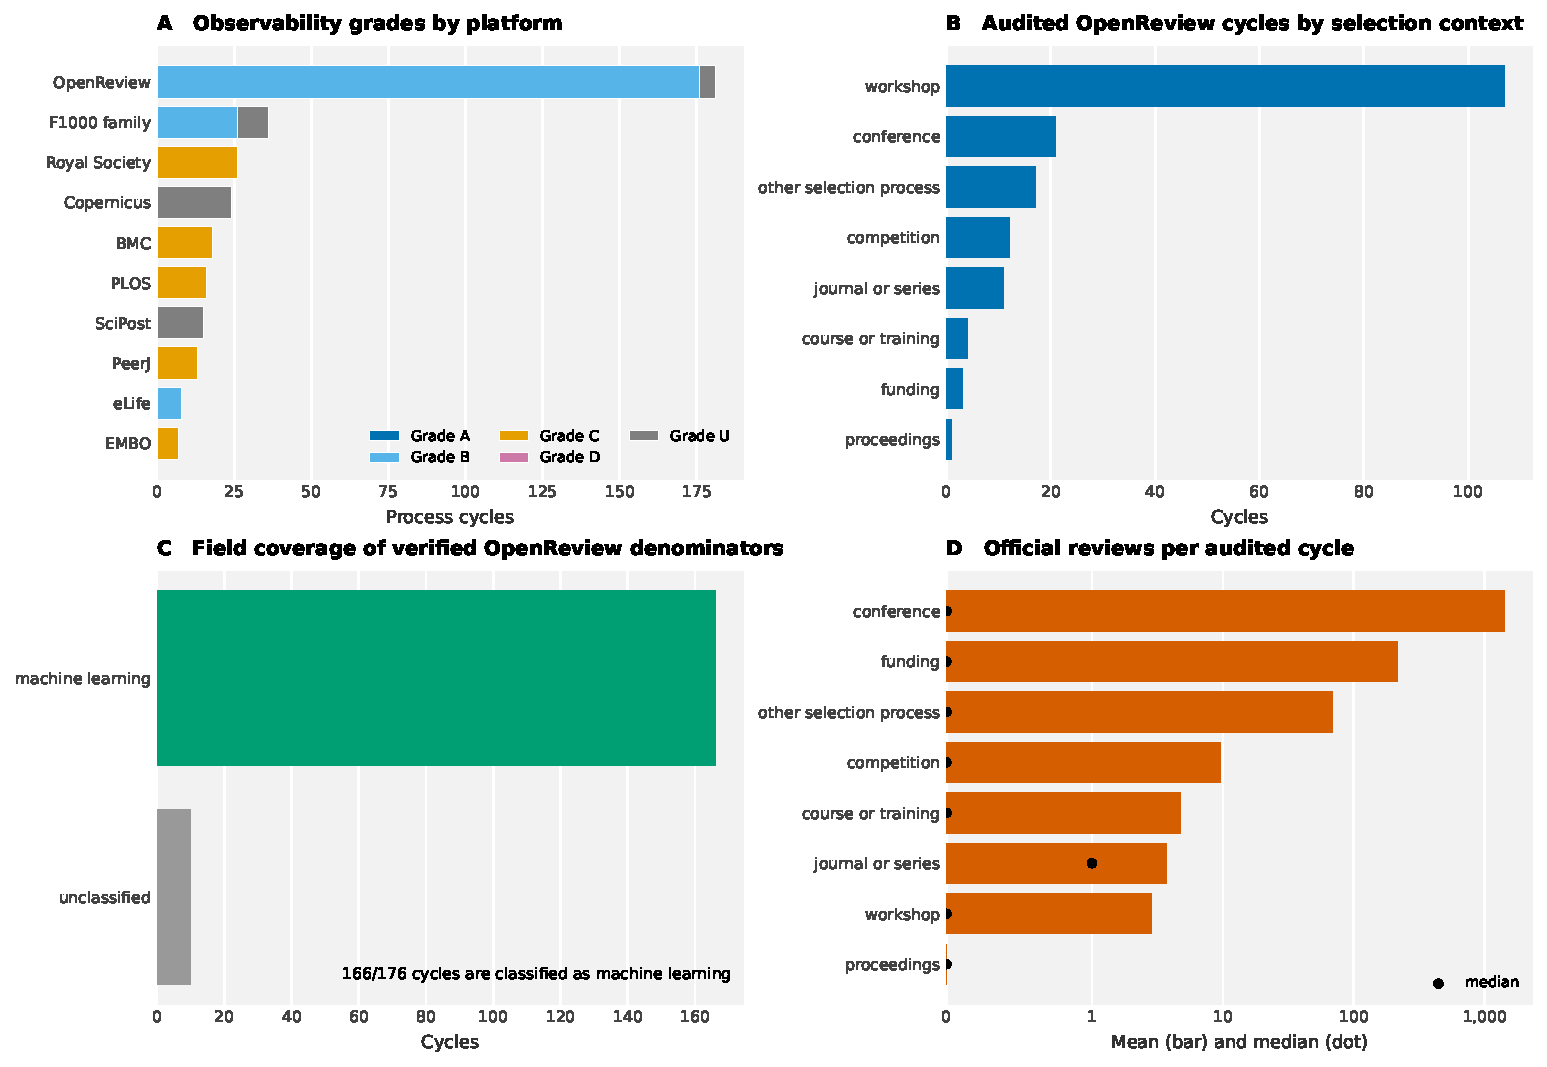
\includegraphics[width=\textwidth]{osg_descriptive_overview.pdf}
\caption{Scale and composition of the process-level analytical release. Panel A separates observability grades by platform. Panels B--D describe the 176-cycle provider-audited OpenReview cohort by selection context, field coverage, and official-review volume. Review volume is concentrated in three large ICLR conference cycles. The figure therefore reports means and medians; the median across all audited cycles is zero, and 38 cycles contain at least one official review.}
\label{fig:descriptive-overview}
\end{figure*}

\subsection{Data model and identifiers}\label{data-model-and-identifiers}

\subsubsection{Core graph}\label{41-core-graph}

The canonical model contains 24 schema artefacts plus a SQL schema and
catalogue. Its central relationships are summarised below; each arrow
denotes a one-to-many relation unless the schema records a many-to-many
link explicitly.

\begin{quote}\small\ttfamily
gate $\rightarrow$ gate\_cycle $\rightarrow$ policy\_version\\
gate\_cycle $\rightarrow$ coverage\_observation, capacity\_observation\\
gate\_cycle $\leftrightarrow$ candidate\_gate\_event $\leftrightarrow$ candidate\\
candidate $\rightarrow$ candidate\_version $\rightarrow$ evaluation,
decision\_event, content\_artifact\\
candidate $\rightarrow$ lineage\_edge, downstream\_outcome\\
source\_object $\rightarrow$ provenance\_event
\end{quote}

\IfFileExists{docs/observatory/figures/osg_er_diagram.tex}
  {\begin{figure*}[t]
\centering
\resizebox{\textwidth}{!}{%
\begin{tikzpicture}[
  node distance=7mm and 10mm,
  entity/.style={draw=MidnightBlue, rounded corners=2pt, fill=MidnightBlue!6,
    minimum height=7mm, inner xsep=5pt, font=\sffamily\footnotesize, align=center},
  event/.style={draw=ForestGreen, rounded corners=2pt, fill=ForestGreen!7,
    minimum height=7mm, inner xsep=5pt, font=\sffamily\footnotesize, align=center},
  evidence/.style={draw=BurntOrange, rounded corners=2pt, fill=BurntOrange!8,
    minimum height=7mm, inner xsep=5pt, font=\sffamily\footnotesize, align=center},
  domainnode/.style={draw=Plum, dashed, rounded corners=2pt, fill=Plum!5,
    minimum height=7mm, inner xsep=5pt, font=\sffamily\scriptsize, align=center},
  link/.style={-{Latex[length=2mm]}, semithick, draw=black!65},
  many/.style={font=\sffamily\scriptsize, fill=white, inner sep=1pt},
]
\node[entity] (gate) {Gate};
\node[entity, right=of gate] (cycle) {Gate cycle};
\node[entity, above right=of cycle] (policy) {Policy version};
\node[evidence, below right=of cycle] (coverage) {Coverage observation\\\scriptsize grade, stage, expected/found};
\node[event, right=17mm of cycle] (cge) {Candidate--gate event};
\node[entity, above right=of cge] (candidate) {Candidate};
\node[entity, right=of candidate] (version) {Candidate version};
\node[event, below right=of version] (evaluation) {Evaluation};
\node[event, below=of version] (decision) {Decision event};
\node[event, above right=of version] (lineage) {Lineage edge\\\scriptsize declared or probabilistic tier};
\node[event, right=of version] (outcome) {Downstream outcome};
\node[evidence, below=15mm of cge] (source) {Source object};
\node[evidence, right=of source] (provenance) {Provenance event};
\node[evidence, right=of provenance] (fieldprov) {Field provenance};
\node[domainnode, above=11mm of gate] (funding) {Funding instrument / round\\\scriptsize eligible pool, panel, allocation};
\node[domainnode, below=11mm of gate] (patent) {Patent application / action\\\scriptsize claims, grounds, amendment, outcome};

\draw[link] (gate) -- node[many,above]{1:n} (cycle);
\draw[link] (cycle) -- node[many,sloped,above]{n:1} (policy);
\draw[link] (cycle) -- node[many,sloped,below]{1:n} (coverage);
\draw[link] (cycle) -- node[many,above]{1:n} (cge);
\draw[link] (candidate) -- node[many,sloped,above]{1:n} (cge);
\draw[link] (candidate) -- node[many,above]{1:n} (version);
\draw[link] (version) -- node[many,sloped,above]{1:n} (evaluation);
\draw[link] (version) -- node[many,left]{1:n} (decision);
\draw[link] (version) -- node[many,above]{1:n} (outcome);
\draw[link] (candidate) -- node[many,sloped,above]{n:m} (lineage);
\draw[link] (lineage) -- (outcome);
\draw[link] (source) -- node[many,above]{1:n} (provenance);
\draw[link] (provenance) -- node[many,above]{1:n} (fieldprov);
\draw[link] (fieldprov) |- (evaluation);
\draw[link,dashed,draw=Plum] (funding) -- (gate);
\draw[link,dashed,draw=Plum] (patent) -- (gate);
\end{tikzpicture}
}
\caption{Entity--relationship view of OSG. Candidate--gate events connect research objects to institutional cycles; coverage observations determine which denominators and rates are admissible. Funding rounds and patent prosecution are represented as domain-specific realisations of the same gate--candidate--event pattern without erasing their native stages or legal meanings. Every normalised fact remains traceable to source and field-level provenance.}
\label{fig:er-diagram}
\end{figure*}
}
  {\begin{figure*}[t]
\centering
\resizebox{\textwidth}{!}{%
\begin{tikzpicture}[
  node distance=7mm and 10mm,
  entity/.style={draw=MidnightBlue, rounded corners=2pt, fill=MidnightBlue!6,
    minimum height=7mm, inner xsep=5pt, font=\sffamily\footnotesize, align=center},
  event/.style={draw=ForestGreen, rounded corners=2pt, fill=ForestGreen!7,
    minimum height=7mm, inner xsep=5pt, font=\sffamily\footnotesize, align=center},
  evidence/.style={draw=BurntOrange, rounded corners=2pt, fill=BurntOrange!8,
    minimum height=7mm, inner xsep=5pt, font=\sffamily\footnotesize, align=center},
  domainnode/.style={draw=Plum, dashed, rounded corners=2pt, fill=Plum!5,
    minimum height=7mm, inner xsep=5pt, font=\sffamily\scriptsize, align=center},
  link/.style={-{Latex[length=2mm]}, semithick, draw=black!65},
  many/.style={font=\sffamily\scriptsize, fill=white, inner sep=1pt},
]
\node[entity] (gate) {Gate};
\node[entity, right=of gate] (cycle) {Gate cycle};
\node[entity, above right=of cycle] (policy) {Policy version};
\node[evidence, below right=of cycle] (coverage) {Coverage observation\\\scriptsize grade, stage, expected/found};
\node[event, right=17mm of cycle] (cge) {Candidate--gate event};
\node[entity, above right=of cge] (candidate) {Candidate};
\node[entity, right=of candidate] (version) {Candidate version};
\node[event, below right=of version] (evaluation) {Evaluation};
\node[event, below=of version] (decision) {Decision event};
\node[event, above right=of version] (lineage) {Lineage edge\\\scriptsize declared or probabilistic tier};
\node[event, right=of version] (outcome) {Downstream outcome};
\node[evidence, below=15mm of cge] (source) {Source object};
\node[evidence, right=of source] (provenance) {Provenance event};
\node[evidence, right=of provenance] (fieldprov) {Field provenance};
\node[domainnode, above=11mm of gate] (funding) {Funding instrument / round\\\scriptsize eligible pool, panel, allocation};
\node[domainnode, below=11mm of gate] (patent) {Patent application / action\\\scriptsize claims, grounds, amendment, outcome};

\draw[link] (gate) -- node[many,above]{1:n} (cycle);
\draw[link] (cycle) -- node[many,sloped,above]{n:1} (policy);
\draw[link] (cycle) -- node[many,sloped,below]{1:n} (coverage);
\draw[link] (cycle) -- node[many,above]{1:n} (cge);
\draw[link] (candidate) -- node[many,sloped,above]{1:n} (cge);
\draw[link] (candidate) -- node[many,above]{1:n} (version);
\draw[link] (version) -- node[many,sloped,above]{1:n} (evaluation);
\draw[link] (version) -- node[many,left]{1:n} (decision);
\draw[link] (version) -- node[many,above]{1:n} (outcome);
\draw[link] (candidate) -- node[many,sloped,above]{n:m} (lineage);
\draw[link] (lineage) -- (outcome);
\draw[link] (source) -- node[many,above]{1:n} (provenance);
\draw[link] (provenance) -- node[many,above]{1:n} (fieldprov);
\draw[link] (fieldprov) |- (evaluation);
\draw[link,dashed,draw=Plum] (funding) -- (gate);
\draw[link,dashed,draw=Plum] (patent) -- (gate);
\end{tikzpicture}
}
\caption{Entity--relationship view of OSG. Candidate--gate events connect research objects to institutional cycles; coverage observations determine which denominators and rates are admissible. Funding rounds and patent prosecution are represented as domain-specific realisations of the same gate--candidate--event pattern without erasing their native stages or legal meanings. Every normalised fact remains traceable to source and field-level provenance.}
\label{fig:er-diagram}
\end{figure*}
}

Additional tables represent identifier aliases, authorship observation,
identity visibility, fields, references, language derivatives, and
field-level provenance. Canonical IDs are deterministic namespaced
UUIDv5 values. Stable native identifiers are inputs where available;
content hashes or deterministic compound keys are used otherwise.
Reharvesting preserves the ID. Uncertain same-work relations remain
evidence-bearing edges with direction, confidence, and linkage tier.

\subsubsection{Provenance and
storage}\label{42-provenance-and-storage}

Raw objects are immutable, compressed, and content-addressed. Retrieval
manifests record source, native identifier, query, retrieval time, byte
hash, connector version, and checkpoint state. Large inactive raw
sources can be packed into append-only indexed containers only after
every member is verified before and after packing. Normalised data are
partitioned Parquet; DuckDB exposes append-only history views and
deterministic current views.

Every normalised fact links to a \texttt{source\_object\_id} and
\texttt{provenance\_event\_id}. Coherent field groups additionally link
through \texttt{field\_provenance} to a source path or JSON pointer,
parser version, confidence, and override history. Tombstones record the
prior existence of a removed object and omit its payload.

\subsubsection{Acquisition and
checkpoints}\label{43-acquisition-and-checkpoints}

All adapters implement the same contract: discover, count, fetch,
checkpoint, normalise, validate a fixture, and emit coverage. Supported
transports include REST cursors and pages, OAI-PMH, JSONL/CSV bulk data,
XML/JATS, HTML, sitemaps, and PDFs. Per-host concurrency, cache reuse,
conditional requests, \texttt{Retry-After}, bounded exponential backoff,
daily request ceilings, and explicit user-agent identification are
mandatory.

Before a population pull, an adapter must pass a deterministic fixture,
source-card, terms/licence review, independent count method, dry run,
and resource estimate. Checkpoints atomically retain the source query,
cursor or page token, last native ID, row count, and shard hash. Forced
interruption tests compare restarted output with uninterrupted canonical
output.

OpenReview required additional safeguards because venue semantics are
invitation-specific and the public APIs expose both current Notes and
Edit histories. The final acquisition used five disjoint domain-history
shards and five contiguous current-Note forum ranges. A union hash,
per-shard run manifests, independent provider totals, and a forum sample
were verified before inclusion in the analytical atlas.

\subsection{Derived products}\label{derived-products}

\subsubsection{Institutional regimes and flow
series}\label{51-institutional-regimes-and-flow-series}

The institutional archive contains one policy observation for each of
\OSGClaimInstitutionalGateCycles{} locally reconstructed gate-cycle rows.
An explicit unknown observation represents the absence of a dated
policy. Current undated pages support current-state description only.
The historical archive contains
\OSGClaimHistoricalPolicyVersions{} policy-version rows.
Machine-readable OpenReview
configuration contributed \OSGClaimOpenreviewRuleRecords{} rule records, and
the rubric crosswalk contains \OSGClaimRubricFields{} native criterion-field
rows.

The flow series adds 176 provider-audited OpenReview cycles and records
observable, reviewed, withdrawn, rejected, selected, and unresolved
counts together with provider expected/found counts, coverage grade,
hidden-stage note, and identity checks. Candidate-denominator validity,
review-incidence eligibility, and selection-rate eligibility are
separate fields. Stage-flow violations cause exclusion or downgrade.

\subsubsection{Evaluations and construct
atlas}\label{52-evaluations-and-construct-atlas}

The release contains \OSGClaimEvaluationObjects{} normalised evaluation
objects, of which \OSGClaimExactEvaluationJoins{} join to an exact candidate
version and gate.
Evaluation kinds include peer reviews, editorial or meta-evaluations,
and other evaluation objects. Official, non-official, and unspecified
statuses are separate fields. Public comments retain their native
classification.

Native rubric values round-trip exactly. Within-cycle calibrated values
are additional fields, and native scales remain available. The
construct layer represents \OSGClaimConstructAtlasConstructs{} broad
human-evaluation constructs and \OSGClaimConstructAtlasRulers{} available
ruler families in \OSGClaimConstructAtlasSelectors{} selector rows.
Construct-bearing spans are released for explicit native criterion
labels. A deterministic research-team audit assessed
\OSGClaimConstructSpanAuditN{} such labels with observed precision
\OSGClaimConstructSpanPrecision{} and a Wilson 95\% lower bound of
\OSGClaimConstructSpanPrecisionLower{}.

Free-form interpretation is evaluated separately against Peer Review
Analyze 1.0 {[}22{]}. A frozen Qwen3 representation and class-balanced
logistic models are evaluated in five folds grouped by submission over
\OSGClaimHumanReviewSpans{} human-annotated spans. The five construct AUCs
range from \OSGClaimHumanReviewMinAuc{} to
\OSGClaimHumanReviewMaxAuc{}. Only out-of-fold probabilities and metrics
are retained. Review prose and embeddings are excluded from the release
and from training of the explicit-rubric crosswalk. The AUC range
describes external benchmark performance on ICLR 2018 annotations. OSG
review records carry no free-form construct score.

\subsubsection{Semantic and recombinatorial
novelty}\label{53-semantic-and-recombinatorial-novelty}

Semantic novelty is represented by two independently trained embedding
rulers. AllenAI's SPECTER2 scientific-document encoder {[}20{]} is pinned
to commit \nolinkurl{3447645e1def9117997203454fa4495937bfbd83}. The
general-purpose Qwen3-Embedding-0.6B model {[}21{]} is pinned to commit
\nolinkurl{97b0c614be4d77ee51c0cef4e5f07c00f9eb65b3}. Both encode the same
title and abstract input. Fitting and model selection are independent of
OSG outcomes. Each target year is compared with documents created before
1 January of that year. Each table reports cosine distance to the prior centroid and
nearest prior document, normalised within source--year cells. Manifests
bind the model revision, input and reference-set hashes, embedding
dimension, parameters, and output checksum. Dense vectors and input text
are removed after feature verification.

SPECTER2 yields \OSGClaimSemanticFeatureRows{} rows and Qwen3 yields
\OSGClaimQwenThreeSemanticRows{}; \OSGClaimSemanticRulerSharedRows{} versions
have both rulers.
Their within-source--year centroid percentiles correlate at
\OSGClaimSemanticRulerCentroidSpearman{}. The median absolute percentile
disagreement is \OSGClaimSemanticRulerMedianDisagreement{}. The release
supplies both values and their disagreement as separate fields.
SPECTER2 contributes a
citation-informed scientific training distribution; Qwen3 contributes
an independently trained, instruction-aware text representation. Their
agreement quantifies convergence between rulers. Another
\OSGClaimFutureDatedExclusions{} future-dated records remain in metadata
and are excluded from time-prior corpora.

Recombinatorial novelty follows the prior-combination logic used in
science-of-science research {[}19{]}, operating on resolved cited-work or
identifier pairs. For each target, pair frequencies are computed from prior years
only; the release retains median conventionality, lower-tail novelty,
and new-combination share. \OSGClaimRecombinatorialVersions{} candidate
versions have adequate citation-pair data.

A second recombination ruler operates on deterministic document-internal
lexical elements: normalised tokens and adjacent token pairs. Its
vocabulary-free construction uses no outcome labels.
For each year, element-pair frequencies are drawn only from earlier
documents. It measures \OSGClaimTextualRecombinatorialVersions{} of
\OSGClaimTextualRecombinatorialDocuments{}
eligible versions (\OSGClaimTextualRecombinatorialCoveragePercent{}).
The public table contains counts and scores without phrase text.
Citation and textual recombination remain separate columns because they
describe different opportunity spaces. Their overlap measures
convergence.

Journal-pair and ontology-concept variants require validated journal and
concept resolution, which is absent from the current public reference
records. Their fields retain missing values.

\subsubsection{Lineage and versions}\label{54-lineage-and-versions}

Lineage edges preserve native relation, normalised relation class,
direction, declaration status, confidence, evidence, and linkage tier.
Relations include new version, resubmission, transfer, split, merge,
extension, and related-only. Many-to-many structures are allowed.

The high-precision analysis layer contains only validated
source-declared relations. It achieved observed precision
\OSGClaimLineagePrecision{} on \OSGClaimLineageAuditN{} audited edges with a
Wilson 95\% lower bound of \OSGClaimLineagePrecisionLower{}.
Candidate generation recovered all source-declared benchmark pairs in
the frozen benchmark. Title collisions remain candidate edges. A
parallel recall-oriented tier begins with each version's 11
nearest titles under the revision-pinned Qwen3 encoder and scores title,
abstract, source, and time features. Source-declared relations form
positive examples; similar non-declared pairs form explicitly labelled
proxy hard negatives. Among \OSGClaimProbabilisticLinkageCandidates{} scored
version-pair candidates, \OSGClaimProbabilisticHighRecallPairs{}
pass the declared-positive recall threshold,
\OSGClaimProbabilisticBalancedPairs{} pass the balanced threshold, and
\OSGClaimProbabilisticHighPrecisionPairs{} pass the high-score threshold.
These proxy-labelled scores serve discovery and sensitivity analysis.
Validated source-declared relations define the analysis-grade lineage
tier.

Human evidence is supplied in a separate calibration table from the
PreprintToPaper Gray Zone {[}25{]}. Two annotators gave decisive labels
to \OSGClaimHumanLineageDecisivePairs{} ambiguous pairs and agreed on
\OSGClaimHumanLineageConsensusPairs{}
($\kappa=\OSGClaimHumanLineageKappa{}$). A five-fold
out-of-fold model at the study's title-similarity design point achieves
an AUC of \OSGClaimHumanLineageOofAuc{} using author overlap. The current
OSG public tier lacks that author feature, so the calibration
probabilities remain benchmark-only. This result also identifies author
overlap as a requirement for future transfer.

Self-loops, temporally impossible edges, and graph cycles are
quarantined. The release also contains \OSGClaimSourceDeclaredLineageEdges{}
source-declared lineage rows, \OSGClaimVersionAlignments{} aligned version
pairs, and \OSGClaimCandidateGateChains{} candidate-gate chain rows.

\subsubsection{Downstream observation states and fixed windows}
\label{55-downstream-observation-states-and-fixed-windows}

The downstream panel contains \OSGClaimAfterlifeCandidates{} candidate rows.
It separates source-declared
later-publication edges, public repository links,
corrections/withdrawals, fixed-window citation observations, and
censoring. Publication-link validation achieved observed precision
\OSGClaimPublicationLinkPrecision{} with a Wilson 95\% lower bound of
\OSGClaimPublicationLinkPrecisionLower{}.
Citation windows are emitted for mature rows.
\OSGClaimImmatureOutcomesExcluded{} immature rows retain an ineligible
state.
The observation-window table expands these candidates into
\OSGClaimPublicationObservationWindowRows{} rows at one-, two-, three-,
and five-year horizons, of which \OSGClaimMatureObservationWindowRows{}
meet the corresponding follow-up requirement. These rows describe what
was observable by the snapshot. Exact publication dates are
unidentified, so the table supports fixed-window analysis and excludes
survival-time estimands. Publication linkage uncertainty is represented by \OSGClaimPublicationLinkageBoundRows{}
source--window bounds and capture-fraction scenarios. All
\OSGClaimPublicationEventTimesUnidentified{} candidates without an exact
publication event time retain an unknown publication state.

\subsubsection{Strain, reforms, and architecture
comparisons}\label{56-strain-reforms-and-architecture-comparisons}

Timing products retain UTC-normalised submission, review, response,
decision, revision, and delay measures where timestamps exist; missing
timestamps remain rows with reasons. Evaluator-supply and workload
proxies are aggregated to gate-cycle level. The public release contains
aggregate evaluator measures only. Three policy events satisfy the
frozen reform registry. Other policy differences remain descriptive.

The construct model compares a single common factor, a correlated
multi-trait representation, and a method-separated representation over
complete cases. Reported correlations are uncorrected for reliability,
and stages remain separate. Existing rows are exploratory. Future
confirmatory tests use the frozen holdout registry.

\section{Data records and release
organisation}\label{6-data-records-and-release-organization}

Version 2.0.0 is an immutable release snapshot. It contains
\OSGClaimReleaseParquetTables{} Parquet tables in
\OSGClaimReleaseComponents{} licence-separated components. Tables have
different units, and several are views or derived measurements over the
same underlying objects. Their row counts therefore describe each table
individually.

{\small
\begin{longtable}[]{@{}L{0.16\textwidth}L{0.13\textwidth}L{0.35\textwidth}L{0.26\textwidth}@{}}
\caption{Release components, licences, contents, and exclusions.}\\
\toprule\noalign{}
Component & Licence & Contents & Principal exclusions \\
\midrule\noalign{}
\endhead
\bottomrule\noalign{}
\endlastfoot
\texttt{metadata} & CC0-1.0 & coverage atlas, gate-cycle flows, policy
archives, rubrics, schemas, documentation, benchmark definitions, static
explorer & raw source objects and protected identifiers \\
\texttt{derived\_}\newline\texttt{features} & CC BY 4.0 & evaluations,
semantic/recombinatorial novelty, lineage, downstream observation states, version alignment,
strain, construct, partial-identification, and transport products & source full text, review text,
reconstructive restricted-text features \\
\texttt{funding\_}\newline\texttt{open\_panels} & CC BY 4.0 / OGL 3.0
& UKRI application--panel events and SNSF proposals, votes, and panel
outcomes & names, proposal text, pre-panel entrants, assignment arms \\
\texttt{funding\_}\newline{\footnotesize\texttt{noncommercial}} & CC BY-NC-SA 4.0 & instrument
evaluability, public opportunity/panel/portfolio series, repeat-awardee
lower bounds, grant-output links & applicant microdata, unfunded
proposal text, inferred assignment arms \\
\texttt{patent\_}\newline{\footnotesize\texttt{noncommercial}} & CC BY-NC-SA 4.0 & PANORAMA application,
action-chain, claim-alignment, prior-art and capacity tables plus HUPD
population cells and a hash crosswalk & claim/action text, confidential applications, personnel
rankings \\
\texttt{validation} & CC0-1.0 & machine-readable build, coverage,
linkage, leakage, privacy, licence, and recovery reports & secrets and
protected audit identities \\
\end{longtable}
}

Each package contains \texttt{VERSION.json}, \texttt{VALIDATION.json},
\texttt{PACKAGE.json}, a file-level SHA-256 manifest, schemas, table
counts, and a DuckDB database. Reuse follows the licence assigned to
each component. The deposit bundles are deterministic tar
archives with normalised ownership and timestamps.
The DuckDB database materialises the smaller analytical tables. Very
large censuses, including the full released HUPD boundary population, remain
directly queryable Parquet assets and are enumerated with row counts and
paths in \texttt{PACKAGE.json}; the release verifier checks both storage
modes.

\section{Technical validation}\label{7-technical-validation}

\subsection{Schema, invariants, and
coverage}\label{71-schema-invariants-and-coverage}

Primary and foreign keys, enum domains, temporal ordering, policy
intervals, native/normalised pairing, provenance reachability, licence
flags, stage flows, and graph cycles are validated on fixtures and
release tables. Coverage requires an independent expected-count method
for any A/B population. The source atlas freezes after every registered
acquisition source has coverage evidence and every required export is
present.

The stage/outcome audit checked \OSGClaimStageOutcomeAuditN{} supported
mappings across stratified native outcomes and found observed precision
\OSGClaimStageOutcomePrecision{}, above the prespecified release threshold.
Unsupported values remain native-only. Policy extraction is audited
against dated raw source
evidence; configuration hash, architecture, criteria, effective date,
byte hash, and scale must all agree. Historical change claims use dated
policy evidence.

\subsection{Temporal leakage}\label{72-temporal-leakage}

The temporal validator tests candidate features against decision time,
reference cutoff, identity visibility, and source observation time.
Deliberately contaminated fixtures include final versions, future
citations, and post-decision identity. They must fail. The semantic
builder separately excludes target-year records from their reference
corpora and rejects future-dated source metadata from feature
eligibility.

\subsection{Linkage and
missingness}\label{73-linkage-and-missingness}

Source-declared links are the highest-precision benchmark. Probabilistic
candidates are released separately with three documented thresholds.
Canonical merges use source-declared evidence. Edge and trajectory counts
can be recomputed under strict source-declared, probabilistic
high-recall, balanced, and high-score layers. Missing text, references,
evaluations, outcomes, and identities are profiled by source and format.
Metadata rows remain when content is absent, and every feature family
declares its coverage rule.

Two external human benchmarks test the places where source declarations
alone are insufficient. Peer Review Analyze supplies construct labels
for free-form prose; all predictions are out of fold and grouped by
submission. PreprintToPaper supplies independently annotated ambiguous
lineage pairs, inter-annotator agreement, and a calibrated author-overlap
model. OSG stores these benchmark predictions in separate tables from
the source-declared tiers. Source-declared evidence governs canonical
entities.

Funding and patent extensions have independent population checks. The
UKRI builders reconcile duplicate rows, outcomes, repeated panels, and
choice-set totals against the official workbooks. The SNSF strict-OOXML
parser preserves every expected proposal--voter cell and validates the
six-value grade domain. The patent builder reconciles all
\OSGClaimPatentPilotApplications{} PANORAMA
cases, performs complete claim-state accounting, and audits HUPD overlap
within the shared filing-year window before publishing the crosswalk.

\subsection{Determinism and clean-room
recovery}\label{74-determinism-and-clean-room-recovery}

Semantic novelty, recombinatorial novelty, lineage, version alignment,
and fixed-window outcome artefacts were rebuilt and compared by exact
SHA-256 in the determinism audit. Clean-room recovery reconstructs
registries, schemas, and representative public fixtures from the
released repository in an isolated environment. The test uses no
network access, credentials, pre-existing generated outputs, or
protected raw lake. Full-source recovery is tested separately through
content hashes, retrieval manifests, checkpoints, and provider-specific
refetch recipes. A disaster-recovery
drill verified \OSGClaimSchemaArtifacts{} schema artefacts,
\OSGClaimRecoverySourceCards{} source cards,
\OSGClaimRegisteredEstimands{} registered estimands, and a
representative seven-source normalised partition.

\subsection{Privacy, licensing, and
security}\label{75-privacy-licensing-and-security}

The release scanner checks table schemas and packaged paths for contact
columns, evaluator identifiers, protected authorship identifiers,
raw/cache paths, and restricted content. An adversarial privacy and
licensing audit tested contact leakage, reviewer re-identification
joins, restricted-text reconstruction, licence incompatibility, and
deleted-object recovery. All highest-severity findings were resolved
before release. Removal
simulations propagate a tombstone through normalised objects, features,
views, manifests, and changelogs.

Acquisition credentials enter through ephemeral environment or provider
secret stores. The framework redacts authorisation data and scans
repository history and artefacts. Public-output reproduction uses no
credentials.

\section{Usage notes}\label{8-usage-notes}

\subsection{Choosing a
denominator}\label{81-choosing-a-denominator}

Users should begin with \texttt{gate\_cycle\_descriptive\_atlas} or
\texttt{coverage\_observation}. An entry-selection rate requires Grade A
and all entrants at the gate-entry stage. A stage-conditional rate may
use Grade A or B and must name the public stage. Grade C supports
statements about visible or selected review histories. Grade D supports
portfolio description. Grade U supports source auditing and missingness
research.

Conceptually, a valid stage-conditional query is:

\begin{Shaded}
\begin{Highlighting}[]
\KeywordTok{SELECT}\NormalTok{ gate\_cycle\_id,}
\NormalTok{       selected\_count:}\CharTok{:DOUBLE} \OperatorTok{/}\NormalTok{ observable\_count }\KeywordTok{AS}\NormalTok{ selected\_share}
\KeywordTok{FROM}\NormalTok{ gate\_cycle\_descriptive\_atlas}
\KeywordTok{WHERE}\NormalTok{ effective\_observability\_grade }\KeywordTok{IN}\NormalTok{ (}\StringTok{\textquotesingle{}A\textquotesingle{}}\NormalTok{, }\StringTok{\textquotesingle{}B\textquotesingle{}}\NormalTok{)}
  \KeywordTok{AND}\NormalTok{ descriptive\_rate\_allowed}
  \KeywordTok{AND}\NormalTok{ observable\_count }\OperatorTok{\textgreater{}} \DecValTok{0}\NormalTok{;}
\end{Highlighting}
\end{Shaded}

The result must be described as conditional on the
row\textquotesingle s \texttt{earliest\_public\_stage}. The verified
observable population supplies the denominator.

\subsection{Evaluation and novelty
research}\label{82-evaluation-and-novelty-research}

Evaluation analyses should join \texttt{evaluation\_\allowbreak objects} to the
exact candidate version and inspect \texttt{official\_\allowbreak status}, native
rubric, scale, and policy version. Construct comparisons should join
their reliability ceilings and report uncorrected estimates. Semantic
features should name encoder, model revision, reference cutoff, and
source--year normalisation. When conclusions depend on semantic
distance, users should report SPECTER2, Qwen3, and their disagreement.
Citation and textual recombination require separate coverage
statements. Every novelty measure should name its construct and
reference corpus.

\subsection{Lineage and afterlife
research}\label{83-lineage-and-afterlife-research}

Within-work analyses should use the source-declared validated layer for
high-precision estimates. Studies prioritising recall may select a
published probabilistic threshold, report sensitivity across thresholds,
and propagate linkage uncertainty. Later acceptance reflects endogenous
routing, withdrawal, revision, and survival. Final-version features are
post-treatment relative to an earlier rejection. Unmatched candidates
retain their right-censored state.

\subsection{Funding and patent
research}\label{84-funding-and-patent-research}

Funding estimators should call the evaluability firewall before use.
The UKRI and SNSF proposal tables support panel-stage comparisons. Their
pre-panel populations and randomised allocation arms are unobserved.
Winner-only records support portfolio and award-recurrence description.
Patent process analyses are
conditional on PANORAMA's rejection-to-allowance sample. Population
comparisons must additionally impose the HUPD filing-year, language,
publicity, and utility-application boundary. Legal grounds must remain
separate. Capacity is released at art-unit--year level with small-cell
suppression; personnel ranking is prohibited.

\subsection{Community benchmarks}\label{85-community-benchmarks}

Six non-generative benchmark tasks cover observability classification,
policy/rubric extraction, stage normalisation, version linkage,
construct measurement, and calibrated missingness.
They use source, time, or domain holdouts; exclude final-outcome leakage
and reviewer identities; and require licence-cleared fixtures or rebuild
pointers. Scoring depends only on released or freely rebuildable inputs.

\section{Ethical and legal
considerations}\label{9-ethical-and-legal-considerations}

The project uses public data and involved no recruitment, contact,
intervention, or bespoke agreement with human subjects. Public
availability establishes an acquisition condition. Redistribution and
permitted analyses follow object-level licences and privacy rules.

Anonymous or pseudonymous reviewers face the highest re-identification
risk. Named authors, applicants, editors, and decision makers face
ranking, employment, harassment, and targeting risks. Public packages
therefore exclude evaluator identifiers, direct contact fields,
protected authorship identifiers, raw source objects, and
purpose-irrelevant person-level joins. Evaluator-supply measures are
aggregate. The project prohibits reviewer deanonymisation,
identity-inference joins intended to reveal anonymous persons,
individual productivity or quality ranking, employment or funding
evaluation, harassment, surveillance, automated targeting, and
restricted-text reconstruction.

Licensing is object-specific. Metadata, article text, review text,
responses, policy documents, images, and derived features may carry
different rights even within one provider. The release builder selects
redistribution, pointer/hash, derived-only, or exclusion per object and
separates incompatible components. A hash records provenance. Rights to
retrieve or reconstruct content follow the source licence.

Corrections and takedowns create versioned tombstones and amended
releases. Source platforms and third-party archives retain their own
records. Community corrections enter through evidence-bearing issue
templates, and every change to a canonical fact creates a new provenance
event.

\section{Limitations}\label{10-limitations}

OSG describes populations that become visible in public records. Hidden
screens create selection into observation. No-assumption regions and
capture-fraction scenarios quantify the compatible entry populations;
narrower estimates require a stated substantive assumption.

Source populations vary in architecture, calendar period, size,
selection share, and review intensity. The transport table measures
overlap in these dimensions for every source pair. Domain coverage is
incomplete, and cycle-level policy and disclosure covariates are absent.
The current diagnostics therefore support conditional modelling or
descriptive stratification according to the recorded verdict.

Licence and privacy rules separate the public package from the protected
acquisition lake. The pointer registry makes
\OSGClaimPointerRebuildArtifacts{} omitted objects verifiable under
their source terms. Retrieval and redistribution remain governed by the
provider and object licence.

Semantic and recombinatorial measurements depend on their construct and
reference corpus. SPECTER2 and Qwen3 show moderate rank agreement.
Textual and citation recombination describe different opportunity
spaces. OSG releases the separate scores, their coverage, and their
disagreement. Free-form construct probabilities are confined to the
external ICLR 2018 benchmark; transfer to other fields, languages, or
review architectures requires new validation.

Source-declared lineage defines the analysis-grade tier. The
PreprintToPaper benchmark includes author overlap, a feature absent from
the current OSG public tier. Qwen3 candidate scores consequently remain
a discovery and sensitivity product.

Publication observation windows record maturity, right censoring,
competing withdrawal states, and linkage uncertainty. Exact publication
dates are unavailable, so these tables support fixed-window analyses.
Publications absent from every linked database remain unknown outcomes.

The funding extension covers funded and unfunded panel-stage candidates
and individual votes for the included UKRI and SNSF panels. Pre-panel
applicants, proposal text, and randomised assignment are outside its
scope. The repeated-awardee table gives a lower bound on award
recurrence.

The privacy-minimised HUPD census supplies a comparison population of
\OSGClaimHupdPublicApplications{} published English-language US utility
applications filed from 2004 through 2018. The crosswalk records exact
matches and boundary differences between HUPD and the PANORAMA process
panel. PANORAMA accounts for claim-set transitions. Claim-set change
supplies a timing proxy because applicant response documents are absent.
Legal novelty and scientific novelty remain distinct constructs.

\section{Code availability}\label{code-availability}

The release is generated from public or genuinely free sources without
paid data or model APIs. Adapter, normalisation, validation, release,
and benchmark code is included in the code/metadata component. The
canonical validation and rebuild commands are:

\begin{Shaded}
\begin{Highlighting}[]
\VariableTok{PYTHONPATH}\OperatorTok{=}\NormalTok{src }\ExtensionTok{.venv/bin/python} \AttributeTok{{-}m}\NormalTok{ observatory.cli validate}
\VariableTok{PYTHONPATH}\OperatorTok{=}\NormalTok{src }\ExtensionTok{.venv/bin/python} \AttributeTok{{-}m}\NormalTok{ observatory.cli r1{-}build}
\VariableTok{PYTHONPATH}\OperatorTok{=}\NormalTok{src }\ExtensionTok{.venv/bin/python} \AttributeTok{{-}m}\NormalTok{ observatory.cli r2{-}build}
\VariableTok{PYTHONPATH}\OperatorTok{=}\NormalTok{src }\ExtensionTok{.venv/bin/python} \AttributeTok{{-}m}\NormalTok{ observatory.cli r3{-}build}
\VariableTok{PYTHONPATH}\OperatorTok{=}\NormalTok{src }\ExtensionTok{.venv/bin/python} \AttributeTok{{-}m}\NormalTok{ observatory.cli r4{-}build}
\VariableTok{PYTHONPATH}\OperatorTok{=}\NormalTok{src }\ExtensionTok{.venv/bin/python} \AttributeTok{{-}m}\NormalTok{ observatory.cli r5{-}build}
\VariableTok{PYTHONPATH}\OperatorTok{=}\NormalTok{src }\ExtensionTok{.venv/bin/python} \AttributeTok{{-}m}\NormalTok{ observatory.cli validity{-}build}
\VariableTok{PYTHONPATH}\OperatorTok{=}\NormalTok{src }\ExtensionTok{.venv/bin/python} \AttributeTok{{-}m}\NormalTok{ observatory.cli release{-}validate }\DataTypeTok{\textbackslash{}}
  \AttributeTok{{-}{-}release{-}id}\NormalTok{ open{-}selection{-}graph{-}2.0.0}
\VariableTok{PYTHONPATH}\OperatorTok{=}\NormalTok{src }\ExtensionTok{.venv/bin/python} \AttributeTok{{-}m}\NormalTok{ observatory.cli release{-}build }\DataTypeTok{\textbackslash{}}
\NormalTok{  results/observatory/releases/open{-}selection{-}graph{-}2.0.0}
\VariableTok{PYTHONPATH}\OperatorTok{=}\NormalTok{src }\ExtensionTok{.venv/bin/python} \AttributeTok{{-}m}\NormalTok{ observatory.cli publication{-}bundles}
\end{Highlighting}
\end{Shaded}

The immutable package is identified by release version 2.0.0, source
snapshot 2026-08-23, the version-registry snapshot identifier, the
package manifest, and file-level
SHA-256 hashes. These identifiers allow any copy of the package to be
verified independently.

\section{Data availability}\label{data-availability}

The data records described in this article are contained in the
licence-separated release package accompanying the manuscript. The
package-level \texttt{VERSION.json}, \texttt{PACKAGE.json},
\texttt{VALIDATION.json}, and \texttt{MANIFEST.json} files identify the
snapshot and provide table counts, component licences, and SHA-256
checksums. Pointer-only source material must be retrieved from its
original provider under the provider's terms; the release records the
source identifier, retrieval recipe, and content hash needed to verify
such reconstructions.

\section{Acknowledgements}\label{acknowledgements}

OSG depends on public infrastructure and upstream datasets
maintained by OpenReview, Crossref, OurResearch/OpenAlex, arXiv, Europe
PMC, Copernicus Publications, eLife, F1000-family platforms, SciPost,
transparent-review publishers, public research funders, the United
States Patent and Trademark Office, and the creators of the derived
corpora credited in the release attribution manifest. Upstream
authorship and licences are preserved in machine-readable and
human-readable attribution files.

\section{References}\label{references}

{\scriptsize
\begin{enumerate}
\def\labelenumi{\arabic{enumi}.}
\tightlist
\item
  Kang, D. et al. A Dataset of Peer Reviews (PeerRead): Collection,
  Insights and NLP Applications. \emph{Proceedings of NAACL-HLT 2018},
  1647--1661 (2018). \url{https://doi.org/10.18653/v1/N18-1149}
\item
  Dycke, N., Kuznetsov, I. \& Gurevych, I. NLPeer: A Unified Resource
  for the Computational Study of Peer Review. \emph{Proceedings of ACL
  2023}, 5049--5073 (2023).
  \url{https://doi.org/10.18653/v1/2023.acl-long.277}
\item
  OpenReview. Introduction to Notes.
  \url{https://docs.openreview.net/getting-started/using-the-api/objects-in-openreview/introduction-to-notes}
  (accessed 20 August 2026).
\item
  OpenReview. Introductions to Invitations.
  \url{https://docs.openreview.net/getting-started/using-the-api/objects-in-openreview/introductions-to-invitations}
  (accessed 20 August 2026).
\item
  OpenReview. Introduction to Groups.
  \url{https://docs.openreview.net/getting-started/objects-in-openreview/groups}
  (accessed 20 August 2026).
\item
  Crossref. REST API. \url{https://api.crossref.org} (accessed 20 August
  2026).
\item
  Priem, J., Piwowar, H. \& Orr, R. OpenAlex: A fully-open index of
  scholarly works, authors, venues, institutions, and concepts.
  \emph{arXiv} 2205.01833 (2022).
  \url{https://doi.org/10.48550/arXiv.2205.01833}
\item
  arXiv. Bulk Data Access.
  \url{https://info.arxiv.org/help/bulk_data.html} (accessed 20 August
  2026).
\item
  Europe PMC. Developers. \url{https://europepmc.org/developers}
  (accessed 20 August 2026).
\item
  Copernicus Publications. Public peer review and interactive public
  discussion.
  \url{https://publications.copernicus.org/services/public_peer_review.html}
  (accessed 20 August 2026).
\item
  eLife. Peer review. \url{https://elifesciences.org/about/peer-review}
  (accessed 20 August 2026).
\item
  F1000Research. How it works and developer resources.
  \url{https://f1000research.com/about} and
  \url{https://f1000research.com/developers} (accessed 20 August 2026).
\item
  SciPost. Editorial procedure and public submissions.
  \url{https://scipost.org/submissions/} (accessed 20 August 2026).
\item
  PLOS. Published Peer Review History.
  \url{https://plos.org/resource/open-peer-review/} (accessed 20 August
  2026).
\item
  Austrian Science Fund. FWF Open API. \url{https://openapi.fwf.ac.at}
  (accessed 20 August 2026).
\item
  Swiss National Science Foundation. SNSF Data Portal.
  \url{https://data.snf.ch} (accessed 20 August 2026).
\item
  LG AI Research. PANORAMA patent office-action dataset.
  \url{https://huggingface.co/datasets/LG-AI-Research/PANORAMA}
  (accessed 20 August 2026).
\item
  United States Patent and Trademark Office. Patent examination and
  office-action research datasets.
  \url{https://www.uspto.gov/ip-policy/economic-research/research-datasets}
  (accessed 20 August 2026).
\item
  Uzzi, B., Mukherjee, S., Stringer, M. \& Jones, B. Atypical
  combinations and scientific impact. \emph{Science} \textbf{342},
  468--472 (2013). \url{https://doi.org/10.1126/science.1240474}
\item
  Singh, A., D'Arcy, M., Cohan, A., Downey, D. \& Feldman, S.
  SciRepEval: A Multi-Format Benchmark for Scientific Document
  Representations. \emph{Proceedings of EMNLP 2023}, 5548--5566 (2023).
  \url{https://doi.org/10.18653/v1/2023.emnlp-main.338}
\item
  Zhang, Y. et al. Qwen3 Embedding: Advancing Text Embedding and
  Reranking Through Foundation Models. \emph{arXiv} 2506.05176 (2025).
  \url{https://doi.org/10.48550/arXiv.2506.05176}
\item
  Ghosal, T., Kumar, S., Bharti, P. K. \& Ekbal, A. Peer review
  analyze: A novel benchmark resource for computational analysis of peer
  reviews. \emph{PLOS ONE} \textbf{17}, e0259238 (2022).
  \url{https://doi.org/10.1371/journal.pone.0259238}
\item
  Heyard, R., Ott, M., Salanti, G. \& Egger, M. Rethinking the Funding
  Line at the Swiss National Science Foundation: Bayesian Ranking and
  Lottery. \emph{Statistics and Public Policy} (2022), with individual
  vote data at \url{https://doi.org/10.5281/zenodo.4531160}.
  \url{https://doi.org/10.1080/2330443X.2022.2086190}
\item
  Suzgun, M., Melas-Kyriazi, L., Sarkar, S. K., Kominers, S. D. \&
  Shieber, S. M. The Harvard USPTO Patent Dataset: A Large-Scale,
  Well-Structured, and Multi-Purpose Corpus of Patent Applications.
  \emph{arXiv} 2207.04043 (2022).
  \url{https://doi.org/10.48550/arXiv.2207.04043}
\item
  Badalova, F., Sienkiewicz, J. \& Mayr, P. PreprintToPaper dataset:
  connecting bioRxiv preprints with journal publications.
  \emph{Scientific Data} (2026).
  \url{https://doi.org/10.1038/s41597-026-06867-3}
\end{enumerate}
}

\end{document}
